\documentclass[a4paper,11pt,fleqn,twoside,notitlepage]{report}\usepackage[]{graphicx}\usepackage[]{color}
%% maxwidth is the original width if it is less than linewidth
%% otherwise use linewidth (to make sure the graphics do not exceed the margin)
\makeatletter
\def\maxwidth{ %
  \ifdim\Gin@nat@width>\linewidth
    \linewidth
  \else
    \Gin@nat@width
  \fi
}
\makeatother

\definecolor{fgcolor}{rgb}{0.345, 0.345, 0.345}
\newcommand{\hlnum}[1]{\textcolor[rgb]{0.686,0.059,0.569}{#1}}%
\newcommand{\hlstr}[1]{\textcolor[rgb]{0.192,0.494,0.8}{#1}}%
\newcommand{\hlcom}[1]{\textcolor[rgb]{0.678,0.584,0.686}{\textit{#1}}}%
\newcommand{\hlopt}[1]{\textcolor[rgb]{0,0,0}{#1}}%
\newcommand{\hlstd}[1]{\textcolor[rgb]{0.345,0.345,0.345}{#1}}%
\newcommand{\hlkwa}[1]{\textcolor[rgb]{0.161,0.373,0.58}{\textbf{#1}}}%
\newcommand{\hlkwb}[1]{\textcolor[rgb]{0.69,0.353,0.396}{#1}}%
\newcommand{\hlkwc}[1]{\textcolor[rgb]{0.333,0.667,0.333}{#1}}%
\newcommand{\hlkwd}[1]{\textcolor[rgb]{0.737,0.353,0.396}{\textbf{#1}}}%

\usepackage{framed}
\makeatletter
\newenvironment{kframe}{%
 \def\at@end@of@kframe{}%
 \ifinner\ifhmode%
  \def\at@end@of@kframe{\end{minipage}}%
  \begin{minipage}{\columnwidth}%
 \fi\fi%
 \def\FrameCommand##1{\hskip\@totalleftmargin \hskip-\fboxsep
 \colorbox{shadecolor}{##1}\hskip-\fboxsep
     % There is no \\@totalrightmargin, so:
     \hskip-\linewidth \hskip-\@totalleftmargin \hskip\columnwidth}%
 \MakeFramed {\advance\hsize-\width
   \@totalleftmargin\z@ \linewidth\hsize
   \@setminipage}}%
 {\par\unskip\endMakeFramed%
 \at@end@of@kframe}
\makeatother

\definecolor{shadecolor}{rgb}{.97, .97, .97}
\definecolor{messagecolor}{rgb}{0, 0, 0}
\definecolor{warningcolor}{rgb}{1, 0, 1}
\definecolor{errorcolor}{rgb}{1, 0, 0}
\newenvironment{knitrout}{}{} % an empty environment to be redefined in TeX

\usepackage{alltt}
\setcounter{tocdepth}{3}
\setcounter{secnumdepth}{3}

\usepackage[utf8]{inputenc}
\usepackage[margin=2.5cm]{geometry}
\usepackage{graphicx}
\usepackage[T1]{fontenc}
\usepackage{enumitem}
\usepackage[section]{placeins}
\usepackage{csquotes}
\usepackage[english]{babel}
\usepackage{float}
\usepackage{caption}
\usepackage{makecell}
\usepackage{hyperref}
\usepackage{bm}
\usepackage{newfloat}
\usepackage[linesnumbered,lined,boxed,commentsnumbered]{algorithm2e}
\usepackage{booktabs}
\usepackage{colortbl}
\usepackage{tikz}

\usepackage{amssymb,amsmath,amsthm,amsfonts}
\newtheorem{theorem}{Theorem}

\usepackage{fancyhdr}
\setlength{\headheight}{15pt}

\pagestyle{fancy}
\renewcommand{\chaptermark}[1]{ \markboth{#1}{} }
\renewcommand{\sectionmark}[1]{ \markright{#1}{} }

\fancyhf{}
\fancyfoot[CE,CO]{\thepage}
\fancyhead[LE]{\textit{ \nouppercase{\leftmark}} }
\fancyhead[LO]{\textit{ \nouppercase{\rightmark}} }
%\fancyhead[RE,RO]{Erik Thors\'{e}n, \href{mailto:Ethorsn@gmail.com}{Ethorsn@gmail.com} }
\fancypagestyle{plain}{ %
\fancyhf{} % remove everything
  \renewcommand{\headrulewidth}{0pt} % remove lines as well
  \renewcommand{\footrulewidth}{0pt}
}

\usepackage[citestyle=authoryear,bibstyle=authoryear,natbib=true,backend=bibtex,hyperref=true,maxnames=2]{biblatex}

\bibliography{REFERENCES.bib}

\title{Statistical process control in next-generation sequencing quality control data}
\author{Erik Thors\'{e}n \thanks{Postal adress: Mathematical Statistics, Stockholm University, SE-106 91, Sweden. E-mail: Ethorsn@gmail.com. Supervisors: Taras Bodnar and Johan Dahlberg}}
\date{\today}

\raggedbottom
\IfFileExists{upquote.sty}{\usepackage{upquote}}{}
\begin{document}
\maketitle

\begin{center}
\begin{abstract}
Any production process needs to be able to ensure quality output. This is no different to the large area of sequencing where the quality of the sequenced data needs to be assured. Using next generation sequencing (NGS) quality control data and statistical process control we have provided a way to monitor and detect changes in a sequential process. In this thesis we have considered monitoring the mean vector and covariance matrix of transformed quality control data from a Next Generation Sequencing (NGS) machine. The transformed data was assumed to be generated by a multivariate normal distribution. We monitored the mean vector using Hotelling's $T^2$ statistic and Croisers MCUSUM control chart (cf. \citet{HotellingQC}, \citet{Croiser1988}). To monitor the covariance matrix we made use of properties of the singular Wishart distribution, first suggested in \citet{Bodnar2009}. Change-points were estimated using a two-sample version of Hotelling's $T^2$ statistic when Croisers MCUSUM chart gave a indication of a change. This approach was retrospective approach was suggested by \citet{pignatiello2001estimation}. A simulation study was performed to test how the constructed control charts performed under persistent changes. Hotelling's $T^2$ statistic showed poor results while the MCUSUM quickly detected changes in transformed NGS quality control data. The simulations and control charts where migrated to C++ using the Rcpp package together with OpenMP, a parallel programming model, to increase computational power. As a real world application, the control charts were applied to transformed quality control data from machines of the same sort. The constructed control charts was also applied on transformed quality control data from other HiSeq machines and detected structural differences between these in terms of their quality control data. These differences were discovered in the mean and covariance matrix.    

\end{abstract}
\end{center}
\newpage
\section*{Acknowledgements}
I would like to thank the SNP\&SEQ platform for the opportunity of doing my thesis in their facility. I would also like to thank my two supervisors Taras Bodnar and Johan Dahlberg who supported me in the writing of this thesis. Taras, who had to answer all my questions on statistical process control and multivariate statistical analysis and Johan, who had to describe the procedures of sequencing with detailed instructions on the problem. Without their help, this thesis would not have been possible. Last, but not least, I would like to thank the people at the platform who had to answer all my questions regarding the machines and programming. 
\newpage
\tableofcontents
\chapter{Introduction}
Ensuring the quality of products is of great importance in any production process. The SNP\&SEQ technology platform (SNP\&SEQ) at the Science for Life Laboratory provides state of the art sequencing and genotyping techniques to Swedish researchers. Ensuring that sequenced data is of high quality is therefore no exception to any other production process. Currently, fixed quality limits are in place to decide if a sample passes quality control or not. Questions such as how to decide these fixed quality limits arise. Also, quality limits may not detect persistent changes in the process which manifests inside these thresholds. A process may produce products of lower quality on average, while still being inside the limits. It may also be so that the process produce products whose quality vary more inside these limits, which may not be desirable. The aim of this thesis is to construct statistical models which can detect changes in next generation sequencing quality control data. Both large and transient- as well as persistent and small changes will be considered. Transient changes will be considered in the mean and the persistent will be considered in both the mean and covariance. Also, if we discover a persistent change, we would like to estimate when this change occurred. In this thesis we will use the framework of statistical process control and change point detection to detect changes and estimate change points.

Statistical process control (SPC) provides a framework for monitoring a process in a sequential setting. SPC was initially developed by \citet{WS}. In his book, Shewhart introduced several concepts but we will mainly focus on the control chart. The control chart is a effective and intuitive way of deducing if a monitored process is performing as expected or desired, which we will refer to as the process being in control (IC). Times where the process is not performing as desired will be referred to as out-of-control (OC). 

Control charts consists of a number of components. The realisations from the process is monitored with the use of a charting statistics. If this charting statistic exceeds a pre-specified control limit the process is deemed to be out-of-control. To determine the control limits for the control chart we need to determine the process IC behaviour or rather, the IC parameters. The IC parameters can sometimes be assumed to be known or otherwise be estimated from a sample which represents the process IC behaviour. In the SPC Literature this procedure is usually described as Phase 1, which constitute of deducing or estimating the in control parameters (cf. \citet{Phase1}). In the next phase, Phase 2, we monitor the process, with the help of the control chart. This thesis will focus on Phase 2 monitoring. This includes a simulation study of how the control charts react to OC behaviour and a application on quality control data from next generation sequencing machines. %However, we will explore the data to be used in this thesis in a exploratory data analysis. how we will quantify the IC behaviour . 

%The procedure is common for the construction of any control chart . Phase 1 refers to deducing regular process behaviour, estimation of the parameters of interest and constructing control limits. Phase 2 is mainly about monitoring the process behaviour. We will use this terminology in this thesis as well.  
The area of statistical process control has been researched extensively and continuously refined since the introduction by Shewhart. The cumulative sum (CUSUM) chart and exponential moving average (EWMA) (cf. \citet{ESPAGE}, \citet{EWMA}), are some of these refinements. The CUSUM chart was introduced to answer the issue of detecting a small and persistent change in the mean of a process, which had not been covered in Shewharts book. In this thesis, we will use two multivariate charts to monitor changes in the mean and covariance matrix of a multivariate normal process. These are Hotelling's $T^2$ statistic and Croisers MCUSUM chart presented in \citet{HotellingQC} and \citet{Croiser1988}, respectively. Hotelling's $T^2$ statistic chart have been documented to detect large and transient- while being very poor at detecting small and persistent changes (cf. \citet{Croiser1988}). Hotelling's $T^2$ statistic also provides a natural and theoretical way to specify control limits. Croisers MCUSUM chart will be used as a complement to detect small and persistent changes of the process. Both charts are used to monitor the mean of a multivariate normal distribution. To monitor the covariance matrix we will make use of properties of the singular Wishart distribution. This idea was first introduced in \citet{Bodnar2009}. Last, we will use a change point estimation model to estimate the time of a persistent change. To use a change point estimation model as a retrospectively tool in SPC was originally presented in \citet{pignatiello2001estimation}.

%In \cite{ESPAGE}, concepts such as the average run length (ARL) was introduced as a measure of performance. A run length is the number of steps until a observation appears outside the control limits of the constructed chart. The average run length is how long it takes until  on average. The ARL will be used extensively with other metrics of performance such as the conditional expected delay, later on in this thesis. 

%The charts to be used in this thesis are Hotellings $T^2$ and Croisers MCUSUM chart presented in \cite{HotellingQC} and \cite{Croiser1988}, respectively. This chart is used to monitor changes in the mean of a multivariate normal distribution. To monitor the covariance matrix, we will use properties of the singular Wishart distribution together with Croisers MCUSUM chart. 

The data to be used in this thesis will be considered as multivariate irregular time series. Each observation represent a run of the machine. We will use both terms as a reference to a new observation. There is a number of settings for each machine which provide different quality characteristic but also changes the inherent dimensionality of the problem. The machine may be used on different settings from run to run and it may stand idle from time to time. Therefore, the following assumptions will be made in this thesis; The irregularity will be disregarded and an observation is independent from previous observations. The data to be used in this thesis will be transformed and the transformed data will be assumed to follow a multivariate normal distribution. Before the transformation is performed, those runs which are poor according to today’s quality criteria are removed. A small section, introducing the transformation methods and evaluating the validity of these assumptions is presented in the Appendix.

The in control parameters where estimated from transformed quality control data, from a specific machine. Using these in control parameters, we constructed Hotelling's $T^2$ and Croisers MCUSUM control chart. In a simulation study it was shown that the MCUSUM chart was able to detect persistent and small changes quickly, on average. Hotelling's $T^2$ statistic showed very poor performance in this simulation study. The change-point detection procedure was seen to estimate the change-point well in the case of large changes in the mean and when the in control period was larger or equal to the out-of-control period. The large amount of simulations performed showed \textsf{R}'s computational limitations. As a consequence a large portion of the simulations were implemented in C++ using the Rcpp extension (cf. \citet{Rcpp}) together with OpenMP, a parallel programming model (cf. \citet{OpenMP}), to further increase computational power.

When applying the control charts to transformed quality control data from other machines, of the same sort, the chart showed the following results. Hotelling's $T^2$ statistic gave a good indication that the different settings of the machines give different quality characteristics. Also, according to Hotelling's $T^2$ statistic the in control parameters fit the other machines transformed quality control data with runs on the same setting. However, Croisers MCUSUM control chart showed large evidence that the estimated in control parameters do not fit the other machines transformed quality control data. In other words, the machines does not perform the same in terms of their transformed quality control data. One should note that this may be a result of the transformation procedures which were used in this thesis.


%The performance of a process is of course not only limited to location shifts but can also include scale parameters. A natural extension to multivariate case is to monitor the mean vector and covariance matrix. 
 %In the literature it is often assumed that the observations are independent and identically normally distributed, see examples such as . 

%which is more thoroughly presented in \cite{SPCIntro},

%Regardless of what kind of performance we are interested in, we assume that we can quantify this behaviour with its IC state. As soon as the process is not performing as we want, it would go into a Out of Control (OC) state, we would like to be alarmed. The alarm will not be able to provide more detailed information than that the process has gone out of control. It is our mission to act upon it, investigate why this alarm was sounded and seek out the root cause. 

%One could deem it more important to maintain a certain performance production quality in a process or one could also be interested in how much the production quality varies. Using SPC we can monitor both characteristics. 
% where they will be The performance can then be sequentially evaluated 

% ......................

%SPC has the possibility to take prior information into account and can monitor more complex changes. SPC is extensively used in the food industry, which is thoroughly discussed in \cite{SPCfood}. It has also been used in other areas such as surveillance of tomotherapy treatment systems, \cite{SPCTomotherapy}. %and \cite{SPCstate2000}. .........

%The aim of this thesis is to construct a model for SNP\&SEQ which can deduce if a sample is an anomaly with respect to the process regular behaviour, or in other terms that the process is out of control. %\textbf{This model is also to be implemented in Scala}.

\section{Outline}
This thesis will be outlined as follows. First, a brief introduction on next generation sequencing (NGS) and the operational routines at the SNP\&SEQ platform is presented. In this section we introduce next generation sequencing, the variables which are collected when the sequencing is performed. Thereafter a chapter presenting the methods to be used in this thesis is presented. Next, a exploratory data analysis is conducted of the two datasets at our disposal. The chapter after that will present results in form of simulations and an application of HiSeq quality control data. We end this thesis with a discussion.
\section{Next generation sequencing and operational routines at the SNP\&SEQ platform}
This section aims to provide some understanding to Next Generation Sequencing (NGS), the hierarchical structure of data, the quality measurements which are collected when sequencing a sample and how the machines work. All information presented here have been attained from \href{https://support.illumina.com/}{Illuminas website (\today)} (machine manufacturer), through discussion with technicians at the SNP\&SEQ platform or otherwise as cited. 

Next Generation Sequencing (NGS) was introduced in 2005, \citet{NGS}. As described in \citet{NATUREseq}, NGS is a collection of approaches or work flows containing library preparation and sequencing. Here, we will only consider one sequencing procedure, sequencing by synthesis (SBS), which Illumina's machines use. The general work flow with SBS follows the steps seen in Table \ref{NGSWorkFlow} with accompanying Figure \ref{Workflowww}. These two provide a simplification of what is presented in \citet{NGS}. 
\begin{table}[!ht]
\caption{The general workflow using sequencing by synthesis.\label{NGSWorkFlow}}
\begin{enumerate}
\item Library preparation - the DNA sample is randomly fragmented and then prepared for placement on a plate (flowcell).
\item Cluster generation or amplification - the prepared library is loaded onto a plate (flowcell) which has some special features. 
These features together with what is called solid-phase amplification make it possible to clone each fragment placed on the flowcell such that each fragment results in a cluster.
\item Sequencing - the flowcell is placed inside the machine where the sequencing can begin using the SBS technology. 
\item Alignment \& data analysis - the sequenced data and quality variables are extracted. 
\end{enumerate}
\end{table}

The two first steps, library preparation and cluster generation, is performed manually or by a machine. The third step where the sequencing is performed, constitutes of a process where of one of four fluorescent-labelled nucleotides binding to their complementary base pair, contained in the DNA fragment on the flowcell. This process results in a florescent light which can be captured by a camera in the machine. There is a trade-off between cluster generation and sequencing performance. To much cluster generation results in over-clustering and the machine can not distinguish which florescent light appear. On the other hand, a to small amount of cluster generation results in under-clustering and the machine can not detect the florescent light properly.
 
 %There are four steps in sequencing. In short, one first prepares the sample by suitable procedures and thereafter, it is placed on a flowcell. While the prepared sample is on the flowcell we amplify it, creating large clusters of what we want to sequence. This is done in order to increase the ability of the machine to see what is actually on the flowcell. There is a trade-off between how large amplification should be performed and the actual performance of the machine. At the SNP\&SEQ platform these procedures are performed by a human and/or a machine. It all depends on the sample. \textit{No information on who has done what exists}. The sequencing is done by taking pictures of the flowcell at different stages in process. With the help of the created clusters, the bases in the photographs are more easily distinguishable since with the help of these they light up more .........................

Each flowcell has 8 lanes and each of these lanes can provide two reads. Figure \ref{HirStructure} illustrates this hierarchical structure of a flowcell. The measurements made on a lane will in general be worse for Read 2. The camera in the machine emits a light in each step of the sequencing procedure. This light will damage the sample placed on the flowcell. The second reason is that the sequencing procedure takes time. The second read can be performed up to two or three days after the run was started. The quality of the sample can will deteriorate under the sequencing procedure because of the amount of time it is inside the machine. 

Each read provides a measurement of the same cluster but from opposite directions. Between each read, the fragments which are to be sequenced, turns 180 degrees. We can therefore interpret it as read 1 sequence the DNA fragment from the top to the bottom and read 2 sequence the DNA fragment from the bottom to the top. This procedure is performed by the machine with the help of a set of chemicals. The procedure is not deterministic and alignment errors can occur.

When a client provides their sample, they will also specify a number of settings which is to be taken into account for a run. A client will specify which tags corresponds to a certain sample. A tag corresponds to a sequence of base pairs. A flowcell can provide several observations from each read in a given lane, corresponding to the search for different tags. This is seen in Figure \ref{HirStructure}. The number of observations may differ between flowcells. This is the structure of the lowest level in a flowcell, which we will refer to as a flowcells ''tag level''. A higher level exists and at this level only one observation for each read is provided. We will call this level the ''read level''. The client also specifies the number of cycles and lanes/reads to be used in a run. The cycles represents how many times we are repeating the SBS procedure. A higher cycle number implies a longer run time. For some machines, there is only one cycle setting and for others several.

In Table \ref{VariableTable} we can see the quality variables provided by the machines and the data pipeline at SNP\&SEQ. We list what level they are measured on and a very brief description of them. Tag level measurements can be aggregated, by the mean or sum, to receive their respective variable measurements found on read level. This is true to the first decimal. Notice that the completed run cycles are not equal to the actual setting. Therefore we will make the following assumption. A run which has a specific number of completed run cycles had a cycle setting equal to the largest closest possible run setting. Under this assumption we can deduce what type of cycle setting the run was performed on.
\begin{figure}[!ht]
\centering
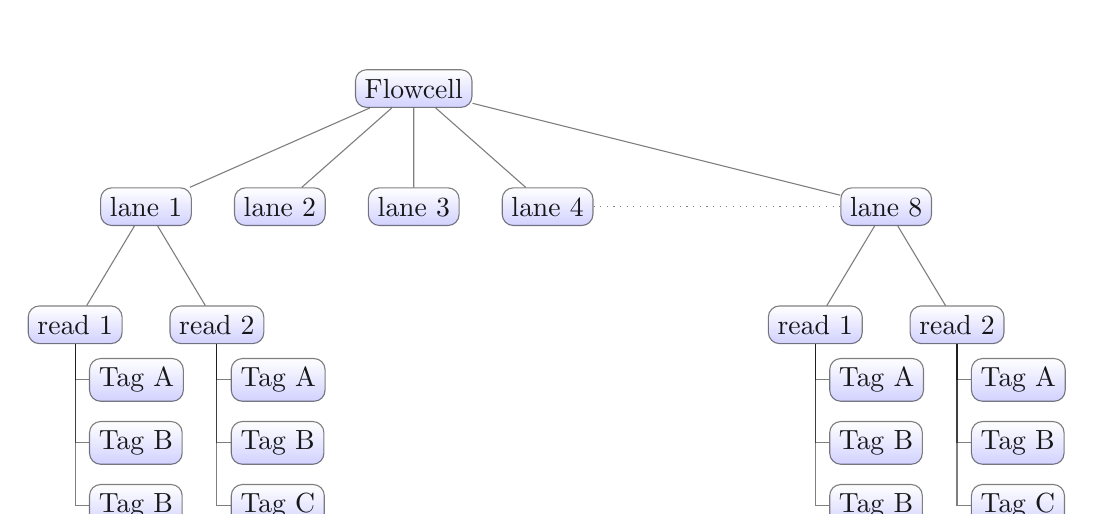
\begin{tikzpicture}[%
	sibling distance=10em,
  	every node/.style = {shape=rectangle, rounded corners,draw,align=center,top color=white, bottom color=blue!20},
    	grandchild/.style={grow=down,xshift=0.5em,anchor=west,
  	  edge from parent path={(\tikzparentnode.south) |- (\tikzchildnode.west)}},
  	grandchildRight/.style={grow=down,xshift=0.5em,anchor=west,
  	  edge from parent path={(\tikzparentnode.south) |-(\tikzchildnode.west)}},
	level 1/.style={sibling distance=17mm},
	level 2/.style={sibling distance=18mm},
	fill opacity=.9,draw opacity=.5
	]
  \node {Flowcell}
    child { node [level 1] (c1) {lane 1} 
    		child [level 2] {node {read 1}
    			child [grandchild, level distance=23mm] { node {Tag B}}	
    			child [grandchild, level distance=15mm] { node {Tag B}}
    			child [grandchild, level distance=7mm] { node {Tag A}}}
    		child [level 2] {node {read 2}
    			child [grandchildRight, level distance=23mm] { node {Tag C}}
    			child [grandchildRight, level distance=15mm] { node {Tag B}}
			child [grandchildRight, level distance=7mm] { node {Tag A}}    		
    		}}
    child [level 1] { node {lane 2} }
	child [level 1] { node {lane 3} }
	child [level 1] { node (c4) {lane 4} }
    child [sibling distance=30mm] { node (c8) {lane 8}
		child [level 2] { node {read 1}
			child [grandchild, level distance=23mm] { node {Tag B}}	
    			child [grandchild, level distance=15mm] { node {Tag B}}
    			child [grandchild, level distance=7mm] { node {Tag A}}}
    		child [level 2] {node {read 2}
    			child [grandchildRight, level distance=23mm] { node {Tag C}}
    			child [grandchildRight, level distance=15mm] { node {Tag B}}
			child [grandchildRight, level distance=7mm] { node {Tag A}}}
    		};
 \draw [dotted] (c4) -- (c8);
		\end{tikzpicture}
 \caption{The hierachical structure of data at the lowest level, tag level, of quality measurement.\label{HirStructure}}
\end{figure}

There are a total of 10 Next Generation Sequencing (NGS) machines of three types (MiSeq, HiSeq2500  and HiSeqX) at the SNP\&SEQ platform. The HiSeqX machines are all of the same model whereas the HiSeq2500 are mixed, upgraded from previous models amongst others. These upgrades do not imply that the machines are equal in terms of their specifications.

Before the NGS machines are used they are cleaned. If a machine is idle for too many days the machine is put through the same maintenance to ensure that it does not deteriorate. It should be noted that the maintenance performed only covers a certain set of parts in the machine such as drain pipes and pumps amongst others. The three different types of machines are generally used for different things. The single MiSeq machine is mainly used for experimental samples. This machine provides less data and the cost of a run is less compared to the others. The MiSeq machine is expected to perform worse since a large portion of variation will be the sample itself. The HiSeq machines are used for common samples and are expected to perform better. They cost more to run but their output is larger. Last, the HiSeqX are the least flexible machines that cost the most to run. These can provide most data amongst the machines and are deemed to be most accurate. 
%When a client is investigating something new or experimental it is often requested to be run on a MiSeq machine. The quality of the sample may be poor because...
\begin{table}[!ht]
\centering
\caption{Table containing quality variables, what level they are measured on and a short description of them. \label{VariableTable}}
\begin{tabular}{lc p{7cm}}
\toprule
Variable & Level & Description \\
\midrule
Mean Q & Tag/Read & The mean quality score of a read \\ 
\midrule
Completed cycles & Tag/Read & Number of completed cycles\\
\midrule
Percent Q30 & Tag/Read & Percentage of base calls which had a Q-value which where over 30 \\ 
\midrule
Error rate & Read & Error rate of read sequence compared to a reference genome  \\ 
\midrule
Percent tag error & Tag & The percent of error of the alignment of this tag \\
\midrule 
Raw cluster & Read & The number of clusters detected in a Read \\ 
\midrule
Past filter Cluster & Tag/Read & The number of clusters detected post filter \\ 
\midrule
Raw Density & Read & The clusters density \\ 
\midrule
Past filter Density & Read & The cluster density, post filter \\
\bottomrule
\end{tabular}
\end{table}

\begin{figure}
\centering
\includegraphics[scale=0.4]{PicSBS.png}
\caption{Figure illustrating the general workflow in sequencing by synthesis. The figure is taken from \citet{NGS}. \label{Workflowww}}
\end{figure}
%The variable \textbf{Mean Q} is the mean of the Phred Q score which is presented in \citet{IlluminaQ}. Without putting to much detail on how the Q score is calculated it is an estimate of how good a cycle is for a specific base. In other words how good the decoding is of a cluster in a picture. As described in Table 1 in the same paper, a Q score of 10 implies a 1 in 10 probability of incorrect base call. A Q score of 30 implies a 1 in 1000 probability of incorrect base call, which is generally deemed as a good and acceptable result. The next variable, completed cycles, is a direct determinant of the machines functionality. Note that these do not represent the actual setting each run was performed on. Since no information was provided on the number of cycles each run was performed on we assume the following; let $R_1$ and $R_2$ represent two cycle settings which suffices $R_1 > R_2$. A run performed on cycle setting $R_1$ can only have at most $R_1$ completed cycles, at least $R_2+1$ completed cycles or zero completed cycles. As an example, a run performed on 126 cycles will have at most 126, at least 102 or 0 completed cycles. A run performed on 101 cycles can at most have 101, at least 52 or 0 completed cycles and so forth. If a run has 0 completed cycles it is assumed to be a malfunction. 

%\textbf{Percent Q30} is the proportion of the sequence of pictures which had a Phred Q score above 30.

\chapter{Methods}
%Statistical process control was initially invented by Walter Shewhart in the 1930s, REF12......
%%%%%%%%%%%%%%%%%%%%%%%%%%%%%%%%%%%%%%%%%%%%%%%%%%%%%%%%%%%%%%%%%
% INTRODUCTION TO METHODS
%%%%%%%%%%%%%%%%%%%%%%%%%%%%%%%%%%%%%%%%%%%%%%%%%%%%%%%%%%%%%%%%%
In this section we will introduce the model, control charts and change-point estimation procedure to be used in this thesis. We begin with introducing our problem, and how we will approach it from a mathematical point of view. After this introduction we continue with the control charts, how to construct them and last the change-point detection procedure.
%As described in \cite{SPCIntro} section 1.3, Phase 1 is primary of exploratory nature. In the literature, it is argued that in Phase 1 one should try to control the process such that it performs optimal or whatever performance that can be considered as in control. In this project, no such thing is possible since the machines at SNP\&SEQ platform cost a lot to run. We will construct a IC sample from all runs performed on these machines up until 2016. From the IC sample we will estimate the IC distributions parameters. 

\section{Problem description}
In Phase 1 we assume that we have observed the target process, which we denote $\{\mathbf{Y}_t\}$. The target process represents what was called the in control state or in control behaviour of the process. It is assumed that realisations from this process are independent and identically distributed according to a $p$-variate normal distribution with mean vector $\boldsymbol{\mu}_0$ and non-singular covariance matrix $\boldsymbol{\Sigma}_0$. The process which generates $\{\mathbf{Y}_t\}$ will be referred to as the in control distribution or in control process. Since independence is assumed we can disregard in which order the observations appear. In this thesis, the parameters are assumed to be unknown and will therefore be estimated using a random sample. Let $\hat{\boldsymbol{\mu}}_0$ and $\widehat{\boldsymbol{\Sigma}}_0$ denote the maximum likelihood estimate based on a random sample $\mathbf{Y}=\{\mathbf{Y}_1,\mathbf{Y}_2,...,\mathbf{Y}_M\}'$ from the in control distribution.

In Phase 2 we consider a sequential p-dimensional process $\{\mathbf{X}_t\}$, which we will refer to as the observed process. If the observed process were to coincide with the target process, that is they share the same distribution, then we will say that the process is in control. On the contrary, if they are do not share the same distribution we refer to the process as being out-of-control. 

We will consider two types of changes, namely transient and persistent changes. Transient changes are those where the observed process shows out of control behaviour but only for a specific observation. The observed process then goes back to the target process. Persistent changes are defined as whenever the observed process departs from the target process and do not return to it. The problem of discovering persistent changes can be placed in a change point framework (cf. \citet{CPDbook}), i.e.
\begin{equation}\label{DefCP}
X_t \sim
\begin{cases} 
\mathcal{N}_p(\boldsymbol{\mu}_0,\boldsymbol{\Sigma}_0), \;\; t<\tau \\
\mathcal{N}_p(\boldsymbol{\mu}_1,\boldsymbol{\Sigma}_1), \;\; t\geq \tau
\end{cases}
\end{equation}
where $\boldsymbol{\mu}_0$, $\boldsymbol{\mu}_1$ are two p-dimensional mean vectors and $\boldsymbol{\Sigma}_0$, $\boldsymbol{\Sigma}_1$ are two non-singular covariance matrices. We will not consider departures from normality. If $\tau<\infty$ then a change occurred at time $\tau$. Thus, up until time $\tau$ the observed process coincides with the target process. In the change point framework, we aim to test \textit{if} as well as \textit{when} a change has occurred.

For these persistent changes, we will consider shifts in the location, i.e. $\boldsymbol{\mu}_0 \neq \boldsymbol{\mu}_1$, and also changes in the covariance matrix of the distribution i.e. $\boldsymbol{\Sigma}_0 \neq \boldsymbol{\Sigma}_1$. However, these changes will not be considered at the same time. Change-points will only be estimated when our models give a indication that the mean has changed.

\section{Statistical process control - SPC}
In this section we will introduce the control charts to be used in this thesis. These are Hotelling's $T^2$ chart and Croisers multivariate cumulative sum (MCUSUM) chart. All charts provide different characteristics and possibilities to detect different behaviour. We will use Hotelling's $T^2$ chart to monitor transient and large changes and MCUSUM to monitor persistent and small changes. 

We will start with introducing Hotelling's $T^2$ statstic for Phase 2 monitoring. Initially, Hotelling's $T^2$ statistic was derived as the generalisation of the univariate one-sample t-test to the multivariate setting where he was first to use the $T^2$ statistic in the multivariate statistical process control (cf. \citet{HotellingQC}). 
%In the multivariate setting, the sample mean vector is compared to the mean vector of a p-dimensional normal distribution. Hotelling's $T^2$ statistic has been investigated thoroughly in the literature  
%These can be known and/or equal or possibly not known nor equal covariance structure. In Phase 2 monitoring we want to test if a new observation comes from the in control distribution with the help of the $T^2$ statistic. 
\subsection{Hotelling's T-square chart}
Let $\mathbf{X}=(\mathbf{X}_1,\mathbf{X}_2,...,\mathbf{X}_M)$ be a random sample from a multivariate normal distribution with mean vector $\boldsymbol{\mu}$ and covariance matrix $\boldsymbol{\Sigma}_0$. We would like to test if the mean vector is equal to $\boldsymbol{\mu}$ is equal to $\boldsymbol{\mu}_0$. The null and alternative hypothesis are 
$$
H_0: \boldsymbol{\mu}=\boldsymbol{\mu}_0 \text{   against   } H_1: \boldsymbol{\mu}\neq\boldsymbol{\mu}_0
$$
Hotelling's $T^2$ statistic is defined as 
$$
T^2 = (M-1)(\bar{\mathbf{X}}-\boldsymbol{\mu}_0)'\widehat{\boldsymbol{\Sigma}}_0^{-1}(\bar{\mathbf{X}}-\boldsymbol{\mu}_0)
$$
where $\bar{\mathbf{X}}$ is the mean vector of $\mathbf{X}$. The statistic can be derived from a likelihood ratio test. The derivation is shown in the Appendix, section \ref{HotDerivation}. In Phase 2 monitoring we observe $\mathbf{X}_t$ one at a time, in a sequential manner. Let $\mathbf{X}_t$ be a observation from the observed process at time point $t$. As presented in \citet{SPCIntro}, section 7.2.2, we Hotelling's $T^2$ statistic for Phase 2 monitoring uses the following charting statistic
$$
T^2_{2,t} = (\mathbf{X}_t-\boldsymbol{\mu}_0)'\boldsymbol{\Sigma}^{-1}_0(\mathbf{X}_t-\boldsymbol{\mu}_0).
$$ 
Under known in control parameters we can interpret the charting statistic $T^2_{2,t}$ as the squared Mahalanobis distance of $\mathbf{X}_t$ to the in control mean vector $\boldsymbol{\mu}_0$, with respect to $\boldsymbol{\Sigma}_0$. Under unknown in control parameters, the in control sample obtained in Phase 1 is used to estimate the in control parameters. By the assumption of independence the in control sample is independent of the observations in Phase 2 monitoring and therefore, the in control parameters are independent of the observed process seen in Phase 2. Hence, the interpretation of $T^2_{2,t}$ does not change. 

Under the assumption that the observed process is in control, $\mathbf{X}_t$ follows the target process. \citet{Tracy1992} showed that under this assumption, 
$$
\frac{(M-p)M}{p(M-1)(M+1)} T^2_{2,t} \sim \mathcal{F}_{p,M-p}
$$
where $\mathcal{F}_{a,b}$ is the F-distribution with parameters $a$ and $b$, $M$ is the sample size of the in control sample and $p$ is the number of parameters. Under a fixed $\alpha$ the control limit $h$ is calculated according to 
\begin{center}
\begin{equation}\label{HotControlLimit}
h=\frac{p(M-1)(M+1)}{(M-p)M}\mathcal{F}_{1-\alpha,p,(M-p)}
\end{equation}
\end{center}
where $\mathcal{F}_{1-\alpha,p,M-p}$ is the $(1-\alpha)\%$ percentile of the $\mathcal{F}_{p,M-p}$ distribution. We signal a alarm if $T^2_{2,t} > h$. 

In the following section we introduce CUSUM chart in the univariate setting and continue on to the multivariate setting. 
\subsection{The cumulative sum (CUSUM) chart}
The univariate CUSUM chart was originally presented by \citet{ESPAGE}. He constructed the CUSUM chart based on what is called the sequential probability ratio test (SPRT). We start with presenting some theory for the ordinary hypothesis testing and then extend it to the SPRT framework. We then introduce the CUSUM chart and show how it is connected to SPRT. 

Let $Z$ denote a continuous random variable distributed according to some distribution $\mathcal{F}$. Let $\mathcal{F}$ have probability density function $f_{\mathcal{F}}$ and $z$ be a realisation from this distribution. As presented in \citet{SeqAnalysis} chapter 1, the regular framework of hypothesis testing considers the null- together with the alternative hypothesis in the following fashion
\begin{align*}\label{nullHyp}
&H_0: Z \sim \mathcal{F}  & \\
&H_1: Z \sim \mathcal{G}. & 
\end{align*}
where $\mathcal{G}$ is some distribution with density $f_{\mathcal{G}}(z)$. The two distributions $\mathcal{F}$ and $\mathcal{G}$ are known and therefore the hypothesis can be tested using a likelihood ratio test. Let 
$$
l(z)=f_{\mathcal{G}}(z)/f_{\mathcal{F}}(z)
$$ 
be the likelihood ratio. Using the single observation $z$ the likelihood ratio can be computed. The value of the likelihood ratio is then compared to a constant $r_1$. If the likelihood ratio, $l(z)$, is larger then the constant $r_1$ we reject the null. If it is less than $r_1$ we fail to reject the null. A sequential probability ratio test introduces a third possibility for intermediate values of $l(z)$. That is, for $r_0<l(z)<r_1$ where $r_0<r_1$, we can neither reject nor fail to reject the null. Intermediate values indicate that we need more information and should therefore continue to observe, or gather, more observations from the process.

Now, let $z_t$ be realisations of the random variable $Z$ at time-point $t$. These realisations are obtained in a sequential order at regular intervals. \citet{ESPAGE} constructed the following charting statistic
\begin{equation}\label{UniCusum}
C_{t}=\max(C_{t-1}+z_t,0)
\end{equation}
where $C_{0}=0$, in order to detect a increase in the mean of the distribution of $Z$. From equation \eqref{UniCusum}, $C_t=0$ when $C_t<\min_{0 \leq i < t} C_i$. Whenever the sequence $C_t$ receives a new minimum, the process resets and starts again from zero. The charting statistic gives a signal of a increase in the mean if $C_{t}>h$ where $h$ is a pre-specified control limit. To see the connection to the SPRT framework we follow \citet{SPCIntro}, section 4.2.4. Assume that $Z$ follows a normal distribution with mean $\mu$ and variance $\sigma^2$. We are interested in testing the hypothesis 
\begin{align*}
&H_0: Z \sim \mathcal{N}(\mu_0,\sigma^2)& \\
&H_1: Z \sim \mathcal{N}(\mu_1,\sigma^2)& 
\end{align*}
or in more compact form $H_0:\mu=\mu_0$ against $H_1: \mu=\mu_1$ where $\mu_0<\mu_1$. Let $\mathbf{z}_t=\{z_1,z_2,...,z_t\}$ represent a random sample of size $t$. The log likelihood ratio can then be written as 
\begin{align}
\log(l(\mathbf{z}_t)) & =  \log(f_{1}(\mathbf{z}_t)/f_{0}(\mathbf{z}_t))  \nonumber \\
					 & = \log\left(\prod_{i=1}^t f_{1}(\mathbf{z}_i)/f_{0}(\mathbf{z}_i) \right) \nonumber \\ 
				     & = \sum_{i=1}^t \log(f_{1}(z_i))-\log(f_{0}(z_i)) \label{loglik}
\end{align}
where the sub-index of the densities $f_i$, $i=0,1$, refers to the distribution under the null and alternative hypothesis, respectively. Using the density of the normal distribution in equation \eqref{loglik} we have that 
\begin{align}
\log(l(\mathbf{z}_t)) &= \sum_{i=1}^t \left( -\frac{(z_i-\mu_1)^2}{2\sigma^2} + \frac{(z_i-\mu_0)^2}{2\sigma^2} \right) \nonumber \\ 
& = \frac{1}{\sigma^2}\sum_{i=1}^t \left(z_i \mu_1-z_i\mu_0-\frac{(\mu_1^2-\mu_0^2)}{2} \right) \nonumber \\
& = \frac{1}{\sigma^2}\sum_{i=1}^t \left(z_i (\mu_1-\mu_0)-\frac{(\mu_1+\mu_0)(\mu_1-\mu_0)}{2} \right)  \nonumber \\
 &= \frac{\mu_1-\mu_0}{\sigma^2}\sum_{i=1}^t \left(z_i-\mu_0 -k\right)
\end{align}
where $k=(\mu_1-\mu_0)/2$. Let 
\begin{align}
\tilde{C}_t	&=\frac{\sigma^2}{\mu_1-\mu_0}\log(l(\mathbf{z}_t))\\ 
			&= \sum_{i=1}^t \left(z_i-\mu_0 -k\right)\\ 
			&= \tilde{C}_{t-1} + (z_t-\mu_0)-k \label{CUSUMUNI}
\end{align}
where $\tilde{C}_0=0$. If we compare the statistic $C_t$, equation \eqref{UniCusum}, to $\tilde{C}_t$, seen in \eqref{CUSUMUNI}, the main difference can be seen in the maximum and the addition of $k$. The maximum can be interpreted as Pages CUSUM chart will never fail to reject the null hypothesis. The CUSUM chart only considers the two options of rejecting the null or what was described as the third option, we need more information. 

A natural extension of the chart suggested in equation \eqref{UniCusum}, under the assumption of normally distributed data, would be to include the constant $k$, which is referred to as the allowance constant (cf. \citet{SPCIntro} section 4.2.2). This implies the following charting statistic
\begin{equation}\label{UniCusum2}
C_{t}=\max(C_{t-1}+z_t-k,0).
\end{equation}
\citet{Moustakides} showed that Pages CUSUM chart is quickest out of all SPRT tests to detect persistent shifts of size $\mu_1-\mu_0=2k$, given a average run length (ARL) and a allowance constant $k$. The in control average run length will be further extended in section \ref{AVERG}. The size of the shifts are seldom known beforehand which implies that $k$ should be chosen such that we detect a \textit{desirable} shift as soon as possible. 

The CUSUM chart was first extended by \citet{Croiser1988} to the multivariate setting from a two-sided univariate chart introduced in \citet{Croiser1986}. We will now introduce Croisers multivariate CUSUM chart presented in 1988. 
\subsubsection{Croisers multivariate CUSUM chart}\label{croiserCUSUM}
The natural and somewhat blunt extension of the univariate CUSUM chart, equation \eqref{UniCusum2}, to the multivariate setting would be to include vector variables in the scheme, i.e. 
\begin{equation}\label{MultCUSUM}
\mathbf{S}_t=\max(\mathbf{S}_{t-1}+(\mathbf{X}_t-\boldsymbol{\mu}_0)-\mathbf{k},0).
\end{equation}
where $\mathbf{X}_t\sim\mathcal{N}_p(\boldsymbol{\mu}_0, \boldsymbol{\Sigma}_0)$. However, deducing which is the largest, a vector or 0, is not trivial nor is it clear how to choose the column vector of allowance constants $\mathbf{k}$. Therefore, \citet{Croiser1988} suggested the following. Consider the vector $\mathbf{k}$, it must have the same direction as $\mathbf{S}_{t-1}+(\mathbf{X}_t-\boldsymbol{\mu}_0)$, or otherwise increasing elements of $\mathbf{k}$ would not shrink $\mathbf{S}_{t-1}+(\mathbf{X}_t-\boldsymbol{\mu}_0)-\mathbf{k}$ towards the zero vector. Also, if we want $\mathbf{k}$ to shrink $\mathbf{S}_{t-1}+(\mathbf{X}_t-\boldsymbol{\mu}_0)$ to $\mathbf{0}$ it will need to have length $k$, i.e. $(\mathbf{k}'\boldsymbol{\Sigma}_0\mathbf{k})^{1/2}=k$. Therefore we set
$$
\mathbf{k}=(k/C_t)(\mathbf{S}_{t-1}+(\mathbf{X}_t-\boldsymbol{\mu}_0))
$$
where $C_t$ is the length of $\mathbf{S}_{t-1}+(\mathbf{X}_t-\boldsymbol{\mu}_0)$ w.r.t. $\boldsymbol{\Sigma}_0$, i.e.
$$
C_t=\sqrt{(\mathbf{S}_{t-1}+\mathbf{X}_t-\boldsymbol{\mu}_0)'\boldsymbol{\Sigma}^{-1}_0(\mathbf{S}_{t-1}+\mathbf{X}_t-\boldsymbol{\mu}_0)
}$$
Now that we have constructed $\mathbf{k}$ in such a way that it will shrink the vector $\mathbf{S}_{t-1}+(\mathbf{Z}_t-\boldsymbol{\mu}_0)$ towards the zero vector, the maximum taken in equation \ref{MultCUSUM} can be seen as setting $\mathbf{S}_t=\mathbf{0}$ whenever $C_t\leq k$. Rather than considering the multivariate CUSUM in equation \eqref{MultCUSUM} we can consider the following, let
\begin{align}
&C_t=\sqrt{(\mathbf{S}_{t-1}+\mathbf{X}_t-\boldsymbol{\mu}_0)'\boldsymbol{\Sigma}^{-1}_0
(\mathbf{S}_{t-1}+\mathbf{X}_t-\boldsymbol{\mu}_0)}\label{MCUSUM} &\\ 
&\mathbf{S}_t=\begin{cases}
\mathbf{0} & \text{if} \; C_t \leq k \\
(\mathbf{S}_{t-1}+\mathbf{X}_t-\boldsymbol{\mu}_0)(1-k/C_t) & \text{ otherwise}
\end{cases} \label{MCUSUM2} &
\end{align}
where $k$ is the allowance constant and $\mathbf{S}_0=\mathbf{0}$. Let 
\begin{equation}\label{Ht}
H_t=\sqrt{\mathbf{S}_t'\boldsymbol{\Sigma}^{-1}_0 \mathbf{S}_t},
\end{equation} 
be the charting statistic. The chart gives a signal if $H_t>h$ where $h$ is a pre-specified control limit. 

\citet{Croiser1988} proved that the chart is directional invariant. It only depends on the non-centrality parameter
$$
\lambda = (\boldsymbol{\mu}_1-\boldsymbol{\mu}_0)'\boldsymbol{\Sigma}_0(\boldsymbol{\mu}_1-\boldsymbol{\mu}_0)
$$
where $\boldsymbol{\mu}_1$ is the out-of-control process mean vector and $\boldsymbol{\mu}_0$ the IC mean vector, defined in equation \eqref{DefCP}. The non-centrality can be interpreted as the statistical distance of the new mean $\boldsymbol{\mu}_1$ to the in control mean. Also, the result implies that we only need to use one chart to monitor all possible changes in the mean vector $\boldsymbol{\mu}_0$. The allowance constant $k$ can be chosen in the same way as described in previous section. 

The choice of $h$ is not trivial and will be extended upon more thoroughly in the section \ref{AVERG}. 

In the next section we will introduce one method for monitoring the covariance matrix, introduced in \citet{Bodnar2009}. They constructed numerous charts for monitoring the covariance matrix based on properties of the singular Wishart distribution.
\subsubsection{Monitoring the covariance matrix using properties of the singular Wishart distribution}\label{Wishartderiv}
% First let us introduce the Wishart distribution together with the singular Wishart distribution. 
Let $\mathbf{X}=(\mathbf{X}_1,\mathbf{X}_2,...,\mathbf{X}_n)'$ be a random sample of size $n$ from $\mathcal{N}_p(\boldsymbol{\mu}_0,\boldsymbol{\Sigma}_0)$. Without loss of generality we may assume that $\mathcal{N}_p(\mathbf{0},\boldsymbol{\Sigma}_0)$. The dimensions of $\mathbf{X}$ is equal to $n \times p$, $n>p$. Let $\mathbf{V}=\mathbf{X}\mathbf{X}'$, then $\mathbf{V}$ follows a p-dimensional Wishart distribution with $n$ degrees of freedom. The $p$ dimensional Wishart distribution, which we will denote $W_p(n,\boldsymbol{\Sigma}_0)$ has the following probability density function (cf. \citet{StatDists}, chapter 47)
\begin{equation}\label{wishartDens}
f(\mathbf{V};\boldsymbol{\Sigma}_0)=\frac{\exp\left(-\frac{1}{2}\mathbf{tr}(\boldsymbol{\Sigma}^{-1}_0\mathbf{V})\right) |\mathbf{V}|^{(n-p-1)/2}}{\Gamma_p(n/2) |2\boldsymbol{\Sigma}_0|^{n/2}}
\end{equation}
where $|\mathbf{A}|$ is the determinant of the matrix $\mathbf{A}$, $\mathbf{tr}(\mathbf{A})$ is the trace of the matrix $\mathbf{A}$ and $\Gamma_p(g)$ is the p-dimensional gamma function. Consider the case where $n<p$, then $\mathbf{V}$ is a rank deficient matrix since
\begin{align*}
&\text{rank}(\mathbf{X})=\min(n,p)=n \; \; &\\
&\text{rank}(\mathbf{V})=\text{rank}(\mathbf{X}\mathbf{X}')\leq \min(\text{rank}(\mathbf{X}),\text{rank}(\mathbf{X}'))=n<p, \;\; \text{with probability one,}&
\end{align*}
by 3.12, \citet{MatrixHandbook}. Also, by the definition of the rank (cf. definition 4.2 \citet{MatrixHandbook}), the matrix $\mathbf{V}$ does not have a inverse and the determinant of the matrix is equal to zero. Under these circumstances, the density in equation \eqref{wishartDens} is zero for all $\mathbf{V}$. The distribution on the other hand, still exists, and do so under the name of the singular Wishart distribution. The properties of the Wishart and singular Wishart distribution was thoroughly investigated in \citet{Bodnar20082389}. These properties was then placed in the multivariate SPC framework in \cite{Bodnar2009}. We will follow their lead in the introduction to monitoring the covariance matrix using properties from the singular Wishart distribution.

 Let $n=1$, then $\mathbf{X}_t$ is a single observation from the p-dimensional observed process. Let $\mathbf{V}_t=\mathbf{X}_t\mathbf{X}_t'$ be the maximum likelihood estimate for the covariance matrix at time point $t$ and partition the matrices $\mathbf{V}_t$ and $\boldsymbol{\Sigma}_0$ in the following way
\begin{align}
\mathbf{V}_t=\begin{pmatrix}
\mathbf{V}_{t;11} & \mathbf{V}_{t;12} \\
\mathbf{V}_{t;21} & \mathbf{V}_{t;22}
\end{pmatrix} & & \boldsymbol{\Sigma}_0=\begin{pmatrix}
\boldsymbol{\Sigma}_{11} & \boldsymbol{\Sigma}_{12} \\
\boldsymbol{\Sigma}_{21} & \boldsymbol{\Sigma}_{22}
\end{pmatrix}.
\end{align}
Note that we removed the subscript 0 when partitioning the covariance matrix. This was done in order to keep the notation readable. Consider the case where $\mathbf{V}_{t;12}$ and $\boldsymbol{\Sigma}_{12}$ are row vectors. For the $i$-th row and column we may reorder $\Sigma_0$ and $\mathbf{V}_t$ such that the element $\boldsymbol{\Sigma}_{11}$ is the $i$-th diagonal element and $\boldsymbol{\Sigma}_{12},\boldsymbol{\Sigma}_{21}$ the $i$-th row and column. Let $\sigma^2_{ii}$ and $\nu_{t,ii}$ be the $i$-th diagonal elements of the covariance matrix $\boldsymbol{\Sigma}_0$ and the matrix $\mathbf{V}_t$, respectively. Let $\boldsymbol{\Sigma}_{21,i}$ and $\mathbf{V}_{t;21,i}$ denote the $i$-th column of $\boldsymbol{\Sigma}_0$ and $\mathbf{V}_{t}$ but without their respective $i$-th element diagonal element. Let $\boldsymbol{\Sigma}_{22,-i}$ denote the $(p-1) \times (p-1)$ matrix without the $i$-th column and row of $\boldsymbol{\Sigma}_0$. The Schur complement (cf. \citet{MatrixHandbook} definition 14.1) for the $i$-th row is defined as
$$
\boldsymbol{\Sigma}^*_{22,-i} = \boldsymbol{\Sigma}_{22,-i} - \boldsymbol{\Sigma}_{21,i}\boldsymbol{\Sigma}_{21,i}'/\sigma^2_{ii}.
$$   
Partition the out-of-control covariance matrix $\Sigma_1$ in equation \eqref{DefCP} in the same manner as above. Let $\Sigma^*_{1;22,-i}$ be the Schur complement for the $i$-th row in the out-of-control scenario. The following theorem was displayed in \citet{Bodnar2009} 
\begin{theorem}
Let $\mathbf{Y}_1, \mathbf{Y}_2,...,\mathbf{Y}_n$ be an i.i.d. $p$ dimensional Gaussian process with $\mathbf{Y}_i\sim \mathcal{N}_p(\mathbf{0},\Sigma_0)$. Let observed process $\{X_t\}$ be defined as
\begin{align}
&X_t \sim
\begin{cases} 
\mathcal{N}_p(\mathbf{0},\boldsymbol{\Sigma}_0), \;\; t<\tau \\
\mathcal{N}_p(\mathbf{0},\boldsymbol{\Sigma}_1), \;\; t\geq \tau.
\end{cases}& \label{obsProc}
\end{align}
Then
\begin{enumerate}[label=(\alph*)]
\item in the in control state 
\begin{equation}\label{etaI}
\boldsymbol{\eta}_{i,t}= \boldsymbol{\Sigma}^*_{22,-i}^{-1/2}\left(\mathbf{V}_{t;21,i}/\nu_{t,ii}-\boldsymbol{\Sigma}_{21,i}/\sigma_{ii} \right)\nu_{t,ii}^{1/2} \sim \mathcal{N}_p(\mathbf{0}_{p-1},\mathbf{I}_{p-1}).
\end{equation}
where $\mathbf{0}_{p-1}$ is the zero vector of length $p-1$ and $\mathbf{I}_{p-1}$ is the $p-1$ dimensional identity matrix.
\item in the out-of-control state 
\begin{align}\label{expect}
& \text{E}[\boldsymbol{\eta}_{i,t}] = (\boldsymbol{\Sigma}^*_{22,-i})^{-1/2} \Omega_i \sigma_ii \frac{\sqrt{2}}{\sqrt{\pi}} & \\
& \text{Var}(\boldsymbol{\eta}_{i,t}) = (\boldsymbol{\Sigma}^*_{22,-i})^{-1/2} \left(\Sigma^*_{1;22,i}+\Omega_i\sigma^2_{ii}(1-2\pi^{-1})\Omega_i' \right)(\boldsymbol{\Sigma}^*_{22,-i})^{-1/2}&
\end{align}
where $\Omega_i = \Sigma_{1;21,i}/\sigma^2_{1;ii}-\boldsymbol{\Sigma}_{21,i}/\sigma_{ii}$.
\end{enumerate}
Moreover, $\{\eta_{i,t}\}$ are independent in the in control and out-of-control state.
\end{theorem}
Part $(a)$ was shown in \citet{Bodnar20082389} and part $(b)$, was shown in \citet{Bodnar2009}. The process $\{\eta_{i,t}\}$ is independent in time if the observed process $\{\mathbf{X}_{t}\}$ is. 

If $\Omega_i=\mathbf{0}_{p-1}$ then no shift has occurred in the covariance matrix of the original observed process $\{\mathbf{X}_{t}\}$. A shift in the covariance matrix would imply a shift in the mean of the transformed quantity in equation \eqref{etaI}. The result provides us with a way to monitor the covariance matrix with methods to monitor changes in the mean of a multivariate normal distribution. Also, if a shift in the mean vector would occur in the observed process in equation \eqref{obsProc} the distribution of $\eta_{i,t}$, $i=1,...,p$ is no longer a $(p-1)$-variate normal distribution. Any control chart which is constructed based on the process $\{\eta_{i,t},\; i=1,...,p\}$ will be sensitive to shifts in the covariance matrix \textit{and} the mean vector of the initial observed process.

In order to monitor the whole covariance matrix we need to use $p$ different charts. As suggested in \citet{Bodnar2009} we define the joint control chart as  
\begin{align}
&C_{i,t}=\sqrt{(\mathbf{S}_{i,t-1}+\boldsymbol{\eta}_{i,t})'(\mathbf{S}_{i,t-1}+\boldsymbol{\eta}_{i,t})} & \\ 
&\mathbf{S}_{i,t}=\begin{cases}
\mathbf{0} & \text{if} \; C_{i,t} \leq k \\
(\mathbf{S}_{i,t-1}+\boldsymbol{\eta}_{i,t})(1-k/C_{i,t}) & \text{ otherwise}
\end{cases} &
\end{align}
where $k$ is the allowance constant and $\mathbf{S}_{i,0}=\mathbf{0}$. Let 
\begin{equation}
H_{i,t}=\sqrt{\mathbf{S}_{i,t}'\mathbf{S}_{i,t}},
\end{equation} 
for $i=1,2,3,...,p$. We define the charting statistic as
$$
H_t = \max(H_{1,t},H_{2,t},...,H_{p,t}).
$$
%where $H_{i,t}$ is the charting statistic based on $\eta_{i,t}$. 
We signal a alarm if $H_t>h$ where $h$ is a pre-specified control limit.

We will now continue with specifying how to determine the control limit $h$ and properly define the average run length. 

%The control limits only need to be determined once, since the random variables $\boldsymbol{\eta}_{i,t}$, $i=1,2,...,p$, are all identically distributed. 

\subsection{Average run length and control limits}\label{AVERG}
In the literature it is often customary to evaluate the performance of the CUSUM or MCUSUM chart using what is called the average run length (ARL). It was first introduced by \citet{ESPAGE} together with the CUSUM chart. It is defined as the average number of observations we can observe in the sequential setting before the chart gives an alarm. Today, literature  differentiate between the in control ARL (ARL$_0$) and the out-of-control ARL (ARL$_1$) (cf. \citet{SPCIntro} or \citet{SPCTomotherapy}). The ARL$_0$ is defined as the average number of observations until the chart gives a alarm when the process is in control. This is closely related to the type 1 error in the regular hypothesis testing framework. The ARL$_1$ represents the average number of observations for the chart to discover a change which is actually present. It is closely related to the power of a test in the regular hypothesis testing framework. 
 
Consider the observed process $\{\mathbf{X}_t\}$ and assume that it is in control. The observed process coincides with the target process. Each observation is assumed to be independent and if the in control parameters are known, the events $H_t > h$, $t=1,2,3,...$, can be seen as independent Bernoulli trials with probability of success $\alpha$. Assume that $h$ is known, $k$ is decided and define the stopping time $N_h$ as the number of independent Bernoulli trials it takes until a successful event, $H_t > h$. The stopping time itself is a random variable which we define as
$$
N_h=\inf\{t\in \mathbb{Z}_+: H_t>h\} \sim \text{ Geo}(\alpha).
$$
The expectation of $N_h$ is by definition equal to the ARL$_0$. If the in control parameters are unknown and estimated from a sample, $N_h$ need not follow a geometric distribution. There will be a dependence between the observations through the estimated parameters. In both cases, to calculate the expectation for a given $h$ is not trivial since the distribution of $H_t$ is not known. However, the distribution need not be known to be able to approximate the expectation of $N_h$. The approximation can be done using Monte Carlo simulation. By the law of large numbers (cf. \citet{LLN} page 172) we have that
$$
\text{E}[N_h] \approx \frac{1}{n} \sum_{i=1}^n N_{h,i}
$$
for large $n$. 

In order to approximate the expectation we need to specify the control limit $h$ and the allowance constant $k$. The Monte Carlo approximation of $\text{E}[N_h]$ using Croisers MCUSUM chart is described in Table \ref{MCAlgo}. The monte carlo approximation is implemented in the functions \texttt{SimulateARL0} and \texttt{SimulateARL0Sigma} which are written in C++ together with OpenMP using the Rcpp extension. OpenMP is a parallell programming model which is written for Fortran, C, C++ and is thoroughly described in \citet{OpenMP}. The Rcpp extension is presented in \citet{Rcpp}. 
\begin{algorithm}
\SetKwInOut{Input}{input}
\SetKwInOut{Output}{output}
\caption{Simulation of the in control average run length, given a control limit $h$ and allowance constant $k$.\label{MCAlgo}}
\SetKwInOut{Initialize}{Initialize}
\Input{A allowance constant $k$, a control limit $h$, the in control parameters $\boldsymbol{\mu}_0$ and $\boldsymbol{\Sigma}_0$}
\Output{A vector with Run lengths}
\BlankLine
\Initialize{$t=0$, $H=0$, $\mathbf{S}_0=\mathbf{0}$}
\While{$H_t<h$ and $t$ is less than some large number}{
Simulate $\mathbf{X}$ from $\mathcal{N}_p (\boldsymbol{\mu}_0, \boldsymbol{\Sigma}_0)$. \\
Calculate $C$ with the help of $\mathbf{S_{t}}$ and $\mathbf{X}$, according to equation \eqref{MCUSUM}. \\
Calculate $\mathbf{S}_t$ according to equation \eqref{MCUSUM2} and then calculate $H_t$. \\
Update $t=t+1$\\
}
Repeat $n$ times.
\end{algorithm}

In order to find the optimal control limit given a target in control average run length, which we refer to as ARL$^*_0$, and a allowance constant $k$, we consider the following function
\begin{equation}\label{FUN}
f(h)=\text{E}[N_h]-ARL^*_0 \approx \left(\frac{1}{n}\sum_{i=1}^{n} N_{i,h}\right)-ARL^*_0.
\end{equation}
We aim to find the $h^*$ which fulfils $f(h^*)=0$. In this thesis, we will use the bisection algorithm described in \citet{NumAnalysis}, page 75, to find such an $h^*$ on a interval $[a_0,b_0]$. In order for the bisection to converge we need to choose a pair $a_0,b_0$ such that $f(a_0)f(b_0)<0$ which can be done by setting $a_0$ relatively small and $b_0$ sufficiently large. However, note that setting $b_0$ large could result in a long time until convergence. The number of simulated run lengths $n$ need to be set equal to a large number to achieve a good estimate of the expectation. The bisection algorithm is implemented in the R function \texttt{CalculateControlLimit}. A outline of the algorithm is presented in Algorithm \ref{hAlgo}. 
\begin{algorithm}
\caption{Bisection algorithm used to find the control limit $h$\label{hAlgo}}
\SetKwData{Left}{left}
\SetKwData{This}{this}
\SetKwFunction{SimulateARL0}{SimulateARL0}
\SetKwInOut{Input}{input}
\SetKwInOut{Output}{output}
\SetKwInOut{Initialize}{Initialize}
\Input{A allowance constant $k$, a interval $[a_0,b_0]$, a target ARL$^*_0$, a maximum number \textbf{Nmax} of iterations, a small number $\epsilon$ and IC parameters $\boldsymbol{\mu}_0$ and $\boldsymbol{\Sigma}_0$}
\Output{Simulated ARL$_0$ for each iteration together with the interval used in that iteration step.}
\BlankLine
	\For{$i \leftarrow 0$ \KwTo \textbf{Nmax}}{
		Set $h_i=(a_i+b_i)/2$ \\
		Use function \texttt{SimulateARL0} or \texttt{SimulateARL0Sigma} to simulate $\text{E}[N_h]$ given $h_{i}$, $k$, $\boldsymbol{\mu}_0$ and $\boldsymbol{\Sigma}_0$.

		\uIf{$|\left(\frac{1}{n}\sum_{i=1}^{n} N_{i,h}\right)-ARL^*_0|<\epsilon$}{
			\textbf{break}, convergence achieved.
		}
		\uElseIf{$\text{ARL}_0<\text{ARL}^*_0$}{
			$a_{i+1}=h_i$ \\
			$b_{i+1}=b_i$
		}
		\Else{
			$a_{i+1}=a_i$ \\
			$b_{i+1}=h_i$		
		}			
	}
\end{algorithm}

In the next section we introduce the change-point detection procedure. The change-point estimation procedure will be used as a retrospective tool for diagnostics when the MCUSUM chart gives a indication of a change. This retrospective change-point estimation procedure was discussed and suggested in the univariate setting by \citet{pignatiello2001estimation}.

\section{Change point estimation}\label{CPDsection}
A CUSUM chart can deliver information indicating that a shift has occurred and also a estimate on when the change occurred. However, \citet{pignatiello2001estimation} proposed the use of a change point detection model to estimate the change point $\tau$, defined in equation \eqref{DefCP}, together with the CUSUM chart. As soon as the CUSUM gave a alarm indicating a change, one would estimate the change point $\tau$ retrospectively. This was done by considering the change point $\tau$ as a parameter of the likelihood and estimating it using maximum likelihood. This proposed method was shown to provide more precise estimates of the change point compared to the estimate from CUSUM charts in a simulation study. 

Consider the model defined in equation \eqref{DefCP}. Let $f_0$ denote the density before the change point $\tau$ and $f_1$ denote the density after the change point. Assume that Croisers CUSUM chart has given a alarm at the $n$th observation in Phase 2 monitoring. Then, we assume that there exists a change point $\tau$ such that $\tau<n$. Let $\mathbf{X}=(\mathbf{X}_1,\mathbf{X}_2,...,\mathbf{X}_n)'$ denote the sample obtained in Phase 2 monitoring. Each observation of the observed process is assumed to be independent and therefore the joint density is equal to
\begin{equation}\label{CPDfun}
f(\mathbf{X},\tau,\boldsymbol{\mu}_1,\boldsymbol{\Sigma}_1) = \prod_{i=1}^{\tau} f_{0}(\mathbf{x}_i;\boldsymbol{\mu}_0,\boldsymbol{\Sigma}_0)\prod_{i=\tau+1}^{n}f_1(\mathbf{x}_i;\boldsymbol{\mu}_1,\boldsymbol{\Sigma}_1).
\end{equation}
The two parameters $\boldsymbol{\mu}_0$ and $\boldsymbol{\Sigma}_0$ are known or have already been estimated and are therefore of no interest to estimate here. We want to estimate the parameters $\tau,\boldsymbol{\mu}_1$ and $\boldsymbol{\Sigma}_1$. First, consider the case where $n<p$. The number of observations obtained in Phase 2 monitoring are less than the number of variables. As described in \citet{CPDbook} section 3.2.1, estimation of the out-of-control covariance matrix $\boldsymbol{\Sigma}_1$ will result in a singular matrix, hence its determinant is equal to zero and by definition the density $f_1(.;\boldsymbol{\mu}_1,\boldsymbol{\Sigma}_1)$ is not defined. Moreover, since the density $f_1(.;\boldsymbol{\mu}_1,\boldsymbol{\Sigma}_1)$ does not exist, the joint density in equation \eqref{CPDfun} does not exist and hence estimation of the change point $\tau$ through a likelihood based procedure is not possible. Now consider the case where $n>p$. In order to estimate a $\boldsymbol{\Sigma}_1$ which must be a non-singular matrix (with probability one) we must consider the case when $p<\tau<n-p$, i.e. the change point would atleast be $p$ steps back in time or atleast $p$ observations past the start of our Phase 2 monitoring. In the case when $p$ is large, the change point can only be estimated far back in time which may not be desirable and in worst case introduce a large bias. Therefore, in this thesis, we will only estimate change points for the mean vector. The density described in equation \eqref{CPDfun} will have parameters $\tau$ and $\boldsymbol{\mu}_1$, i.e.
\begin{equation}\label{CPDfunRed}
f(\mathbf{X};\tau,\boldsymbol{\mu}_1) = \prod_{i=1}^{\tau} f_{0}(\mathbf{X}_i;\boldsymbol{\mu}_0,\boldsymbol{\Sigma}_0)\prod_{i=\tau+1}^{n}f_1(\mathbf{X}_i;\boldsymbol{\mu}_1,\boldsymbol{\Sigma}_0).
\end{equation}
As explained in \citet{CPDbook}, section 3.1.1, we can interpret the situation as a two sample problem. For a given $\tau=\tau_1$, we have two independent samples from two multivariate normal distributions where we would like to test if they share the same mean vector. By this reasoning we can use Hotelling's $T^2$ statistic as a measure of evidence that the change point occurred at the given time point $\tau_1$. The largest value of Hotelling's statistics shows most evidence against the null hypothesis and can be used as a estimator for the change point. 
%We can once more consider the likelihood ratio under the hypothesis 
%$$ 
%H_0: T>n \text{ against } H_1: T<n
%$$
%where the density under the null hypothesis is given by the target distribution and the density under the alternative is given by equation \eqref{CPDfunRed}.
%In  it is suggested to use Hotelling's $T^2$ statistic to estimate the change point $T$.
Hotelling's statistic, derived in Appendix section \ref{HotDerivation}, is done so under the assumption of one sample from a p-dimensional normal distribution. This setting is extended in \citet{MultStatAnalysis}, section 5.3.4 to a two-sample problem where two means from two normal distributions are compared. Here, it is assumed that the covariance matrix are equal but unknown. In this application, the in control parameters are assumed to be known and that some part of the sample may come from the target process. Therefore, we suggest the standardized difference between the in control parameter and the mean of the out of control sample, as done in \citet{MultStatAnalysis} but in the case of a known covariance matrix. The standardized difference is defined as 
$$
\mathbf{y}_{\tau} = \sqrt{\frac{\tau(n-\tau)}{n}}(\boldsymbol{\mu}_0-\hat{\boldsymbol{\mu}}_1(\tau)).
$$
where $\hat{\boldsymbol{\mu}}_1(\tau)=1/(n-\tau)\sum_{i=\tau}^{n} \mathbf{X}_i$ is the maximum likelihood estimator of $\boldsymbol{\mu}_1$ of the density shown in \eqref{CPDfunRed}. We can now construct a two-sample Hotelling's $T^2$ statistic 
\begin{align}
T^2_{\tau}=\mathbf{y}'_{\tau} \boldsymbol{\Sigma}^{-1}_0 \mathbf{y}_{\tau} \;\;\;\;\; \text{for } \tau=1,2,3,...,n-1
\end{align}
and estimate the change point $\tau$ by $T^2_{\hat{\tau}} = \max_{\tau} T^2_{\tau}$.

% As stated in \citet{SomethingOdd}, this estimator maximizes the profile likelihood $L(\tau, \hat{\boldsymbol{\mu}}_1(\tau))$, of the density in \eqref{CPDfunRed}. %This can be shown by considering the maximization of the density in equation \eqref{CPDfunRed} as a linear integer programming problem of the profile likelihood. We will refrain from showing this in this thesis. %The estimated change point can be described as the point in time which maximizes the squared statistical distance between the estimated mean vector $\hat{\boldsymbol{\mu}}_1(T)$ and $\boldsymbol{\mu}_0$.



\chapter{Exploratory data analysis}





In this section we will conduct a exploratory data analysis. We will first introduce the datasets which will be used in this thesis and then continue with exploring them seperately. We will focus our attention to the data of one of each model. 

The data to be used in this thesis consists of two sets. The first set contains observations on the lowest level, what we called tag level. There is no fixed number of tags for each run and therefore each flowcell can contain a different number of measurements. In the tag level dataset, there are a total of $786$ runs (unique flowcells) which have been performed since 2012 up until the end of 2015. 

The second dataset contains observations from what we called read level. There are a total of $801$ runs which implies that there is a difference between the datasets. A total of $15$ runs are missing from the Tag level. The missing runs are from the MiSeq 1, HiSeq 3 and 6 machines. These missing runs will be excluded from the data. Also, runs performed in 2012 was done so under different circumstances. It was advised that data from 2012 was not to be used. Therefore, quality control data from 2012 will be removed from our data set.

In Table \ref{CompCycl} we can see the completed run cycles for the HiSeq (Hi) and HiSeqX (HiX) machines. We can start with noticing that HiSeq 1 and 2 are not present in the table. These have been taken out of production. The HiSeqX machines have all been run on the same cycle setting, with every completed cycle equal to 150. This is the only setting used at the SNP\&SEQ platform for HiSeqX. The HiSeq machines shows a much wider range of completed cycles. This is a consequence of the wide range of settings that have been used. We can see that HiSeq 6 (Hi6) have most runs in the vicinity of 124-125 completed cycles. A cycle setting of 126 is one of the most common cycle settings for HiSeq machines at the SNP\&SEQ platform. We will use this machine to represent the HiSeq machines. As the HiSeqX machines did not differ in the cycle setting we will use the HiSeqX 1 to represent the HiSeqX machines. The MiSeq 1 machine has a wide range of 0-500 completed cycles with a lot of different run settings. Those observations having 0 completed cycles are runs which have been documented to be malfunctions. It was removed to shorten the table but will be included, to some extent, in the exploratory analysis.

The last row in Table \ref{CompCycl} shows the total number of runs performed on each machine. The HiSeq 4 machine has most runs of all but also a large diversity in the run settings. 

% latex table generated in R 3.2.3 by xtable 1.8-2 package
% Tue Mar  1 09:34:31 2016
\begin{table}[!t]
\centering
\caption{Table showing the number of flowcells with a specific number of completed cycles for HiSeq (Hi) and HiSeqX (HiX) machine.} 
\begin{tabular}{lccccccccc}
  \toprule 
  & \multicolumn{9}{c}{Machine} \\ \cmidrule(r){2-10} 
Cycles & Hi3 & Hi4 & Hi5 & Hi6 & HiX1 & HiX2 & HiX3 & HiX4 & HiX5 \\ 
  \midrule
49 & 7 &  &  &  &  &  &  &  &  \\ 
  50 & 16 & 10 & 11 & 7 &  &  &  &  &  \\ 
  60 &  &  &  & 3 &  &  &  &  &  \\ 
  99 & 2 & 4 & 2 & 1 &  &  &  &  &  \\ 
  100 & 73 & 49 & 15 & 6 &  &  &  &  &  \\ 
  124 &  & 22 & 22 & 30 &  &  &  &  &  \\ 
  125 &  & 53 & 46 & 50 &  &  &  &  &  \\ 
  150 & 11 & 2 & 14 & 16 & 30 & 27 & 22 & 32 & 16 \\ 
  200 &  &  &  & 1 &  &  &  &  &  \\ 
  250 & 6 & 1 &  &  &  &  &  &  &  \\ 
  \midrule
  $\Sigma$ & 115 & 141 & 110 & 114 & 30 & 27 & 22 & 32 & 16 \\ 
   \bottomrule
\end{tabular}
\label{CompCycl}
\end{table}

We will now investigate investigate the mean q values of each successive run at a tag level. In Figure \ref{fig:TagLevelTS} we can see the mean of mean q tag level measurements together with the range (min to max) for three different machines of different types for lane 1 stratified on read. The observations are presented in their order of appearance.

For lane 1 measurements, the mean for HiSeq 6 of mean q tag level measurements is very connected to its range. If the range is large then the mean is usually worse. The variability of mean tag level measurements in read 2 is larger compared to measurements made in read 1. HiSeqX is seen to have a small range in each run, for read 1 and 2 measurements. Read 2 measurements are lower on average but do not show any substaintial increase in variance. MiSeq 1 is seen to be the worst of all in terms of its mean q tag level measurements. It is clearly seen in the large variance of the means and the large range in some runs. This was to be expected since the MiSeq machine was used for experimental samples on several different settings. 
\begin{knitrout}
\definecolor{shadecolor}{rgb}{0.969, 0.969, 0.969}\color{fgcolor}\begin{figure}[!htbp]
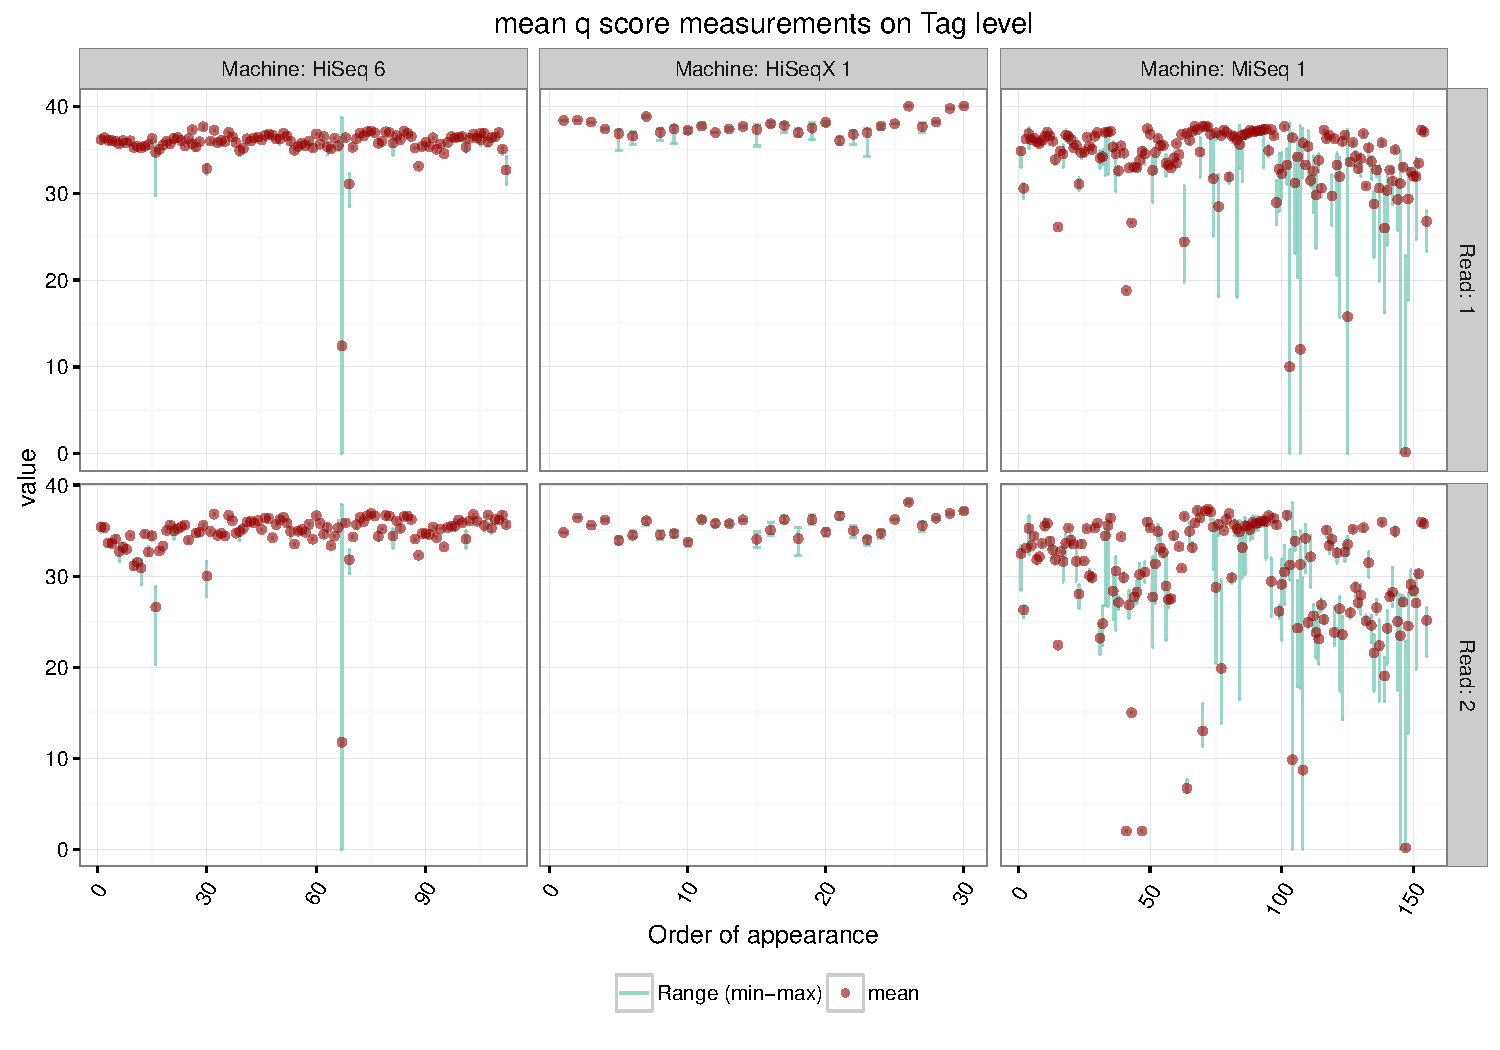
\includegraphics[width=\maxwidth]{figure/TagLevelTS-1} \caption[Figure containing the range (min to max) and mean of each successive run (flowcell)]{Figure containing the range (min to max) and mean of each successive run (flowcell). Here, we are showing read 1 and 2 in lane 1, disregarding what type of setting the run is performed on.}\label{fig:TagLevelTS}
\end{figure}


\end{knitrout}
We will now focus on the HiSeq 6 machine with 102 to 126 completed cycles, in order to make this EDA sufficiently short. 

In Figure \ref{fig:HiSeq6Comb} the range together with the mean of lane 1 and read 1 is shown in their order of appearance. The variables shown here are percent data above a q-score of 30 and the percent tag error. These measurements are from tag level for the HiSeq 6 machine with a cycle setting of 102 to 126. The last figure contains the number of observations in each lane 1 and read 1. %Also, the scale of the percentage is reversed such that both variables graphical interpretation are the same. A low value is not desirable. 
The first variable, the percentage of data above a Q score of 30, which we will refer to as percent Q30, shows a overall small amount of variation. When the spread increases the mean does aswell. The percent tag error can be seen to be very close to zero and at some times equal to zero. This is surprising since the construction of the variable is connected to the error rate. If one is zero, the other should be aswell. However, for \textit{some} runs with zero percent tag error, the error rate is well above zero. We will refrain from using this variable since the quality of it can not be assured. The number of observations contained in lane 1 read 1 varies a lot. It does not seem to relate to the range nor the mean of neither variable.
\begin{knitrout}
\definecolor{shadecolor}{rgb}{0.969, 0.969, 0.969}\color{fgcolor}\begin{figure}[!htb]
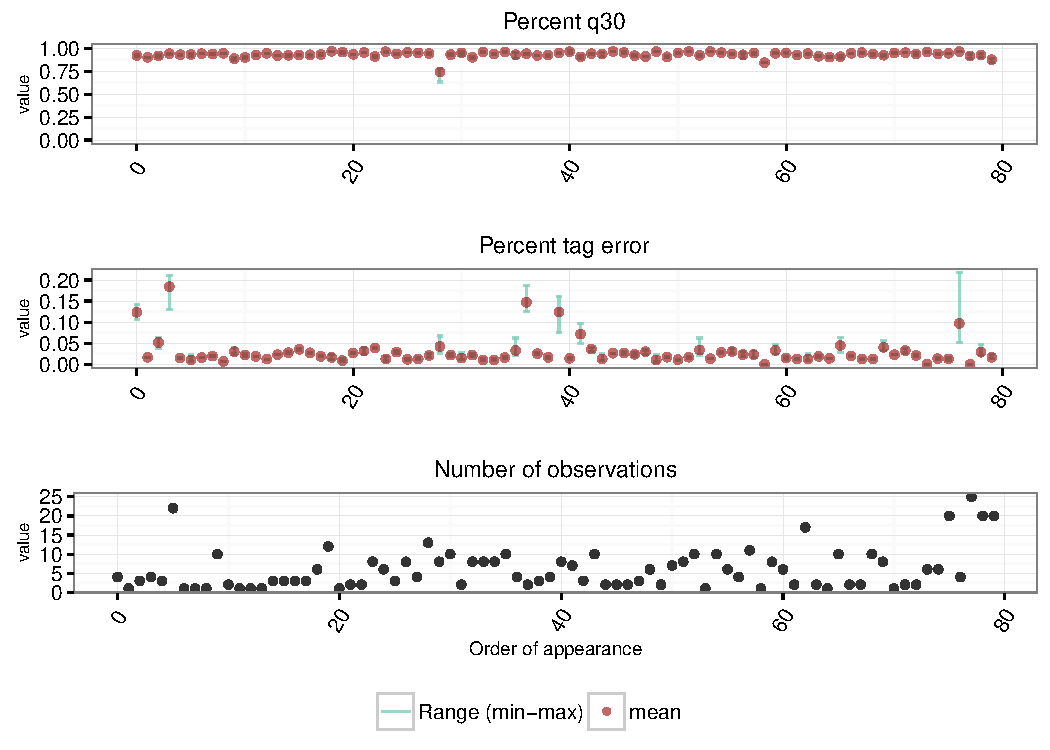
\includegraphics[width=\maxwidth]{figure/HiSeq6Comb-1} \caption[Figure showing the range (min to max) and mean of each succsessive run (flowcell) in lane 1, read 1, of the two variables Percent q30 and Percentage tag error]{Figure showing the range (min to max) and mean of each succsessive run (flowcell) in lane 1, read 1, of the two variables Percent q30 and Percentage tag error. All runs shown where performed on 126 cycles.}\label{fig:HiSeq6Comb}
\end{figure}


\end{knitrout}
We will now investigate what we called the read level measurements. At this level only one observation per read and lane is supplied. We can therefore consider each run as a realisation of a random vector following a multivariate distribution. In this setting we have 7 different variables, with 16 measurements in each. Since the HiSeq 6 machine has been our main interest so far, we will continue in this fashion and compare it to the other HiSeq machines. All runs will henceforth be using all 8 lanes and a cycle setting on 126. The HiSeq 3 machine do not have any runs on this specific cycle setting and will therefore be omitted.

In Figure \ref{fig:MeanVectorFigure} we have the mean together with the range of the error rate variable. We can see that no measurements are zero in this case. The HiSeq 5 machine seems to have a consistently lower error rate compared to the other machines. The HiSeq 6 machine has shown one, or possibly several, runs with large error rates in different lanes. To further investigate the distribution of the error rate together with those variables which have not been looked upon, we will look at them in a histogram.  
\begin{knitrout}
\definecolor{shadecolor}{rgb}{0.969, 0.969, 0.969}\color{fgcolor}\begin{figure}[!htb]
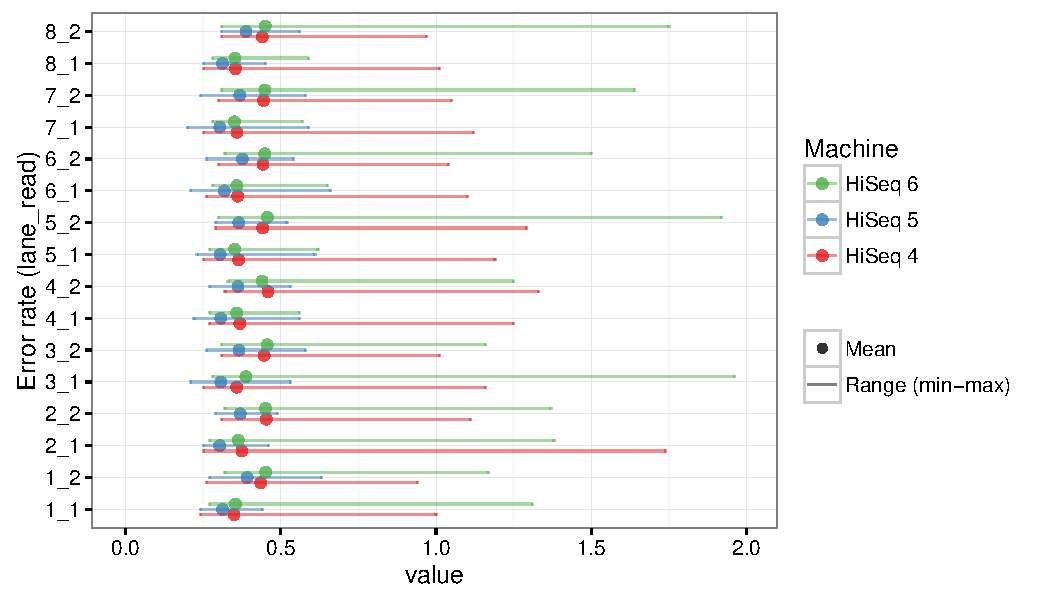
\includegraphics[width=\maxwidth]{figure/MeanVectorFigure-1} \caption[Mean together with the range of the error rate of each lane and read (lane\_read)]{Mean together with the range of the error rate of each lane and read (lane\_read). Notice that the HiSeq 5 has the lowest mean error rate of all HiSeq machines.}\label{fig:MeanVectorFigure}
\end{figure}


\end{knitrout}


In Figure \ref{fig:ReadlvlER} we have a histograms of the error rate, raw cluster density and the number of raw clusters for lane 1 and 2, both reads. In the error rate (row one), we can see that read 2 contains more variability compared to read 1. The distribution of read 1 is more peaked while the distribution for read 2 is quite flat. We can also see that the distribution is somewhat skewed, tending towards the right. For the two later rows, the density and cluster variable can be seen to be close to symmetric. The distribution of the density and cluster variables also look very much alike. 
%Error rate measurements from read 1 can be stable while read 2 deviates. An example can be seen around the 20th observation in the error rate for lane 1. 
%This deviating behaviour is not necessarily seen in any other variable, in the same lane and read. 
%What can be seen in the second and third row is that the raw- density and cluster variables correlate almost perfectly. 
%This is seen in several variables. The following variables is almost perfectly correlated; raw clusters, post filter clusters, raw density, post filter density for each read inside a lane. 
%We will exclude all but the raw clusters variable in the analysis. 
%The raw cluster variable is also almost perfectly correlated for each read inside a lane. This can be seen in Figure \ref{fig:ReadlvlER} when comparing the variables inbetween reads for a given lane. 
%We will remove read 2 for the raw cluster variable in every lane, from the analysis.  
\begin{knitrout}
\definecolor{shadecolor}{rgb}{0.969, 0.969, 0.969}\color{fgcolor}\begin{figure}[!htb]
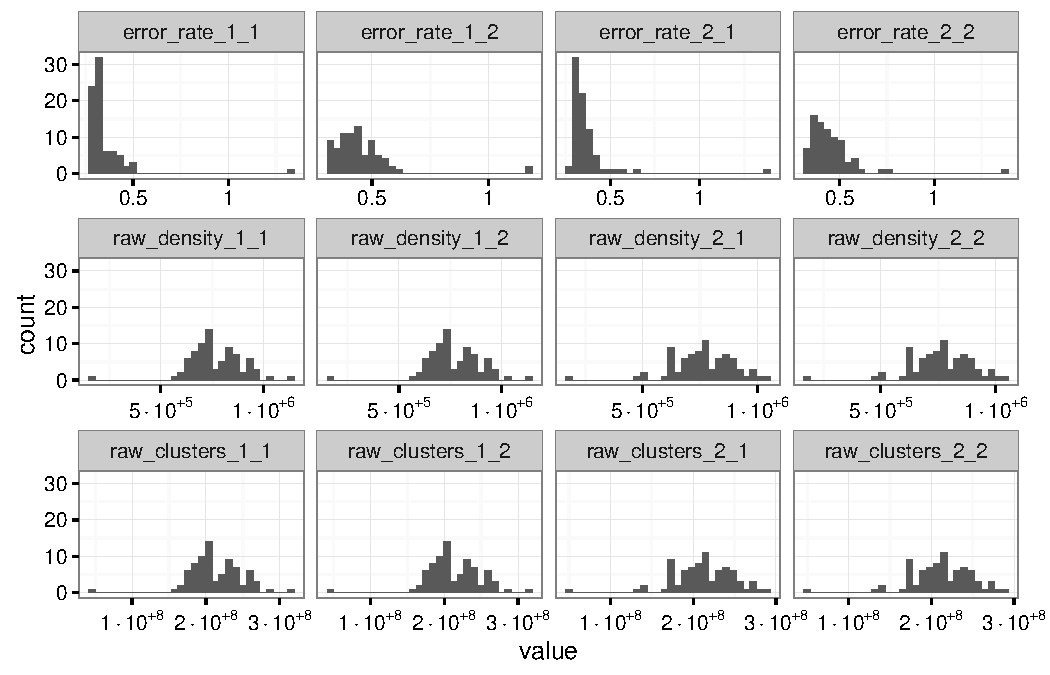
\includegraphics[width=\maxwidth]{figure/ReadlvlER-1} \caption[Error rates, the raw density and the number of raw clusters for each read in lanes 1 and 2]{Error rates, the raw density and the number of raw clusters for each read in lanes 1 and 2. The variable name are listed in the following manner: Variable\_lane\_read.}\label{fig:ReadlvlER}
\end{figure}


\end{knitrout}
The Spearman correlation matrix is visualized in Figure \ref{fig:ReadlvlCor}. The number of variables in the Figure is equal to $112$. The correlation matrix is estimated from a sample size of $213$. In this figure the axis labels where omitted but a header for each group of variables is placed next to them. As an example, the top 16 variables in Figure \ref{fig:ReadlvlCor} corresponds to the error rate for each read and lane which is denoted by the label. We will refer to this as a section of variables. 

We can see that the density and cluster sections of variables correlate almost perfectly. This is especially true for measurements on the same read in a lane. The mean q and percent q30 sections seem to be correlated to each other while not having much correlation to the cluster and density variables. The error rate is negatively correlated with percent q30 and mean q measurements from the same read and lane, while not showing much correlation to other reads and lanes. The correlation matrix can almost be placed on a block diagonal form where three first sections of variables create one block and the last four create another. %Variables on the same read and lane seem to be correlated well while 
%A deviating pattern is is also seen in this section of variables. Those mean q and percent q30 corresponding to lane 7 read 1 and 2, shows much less correlation to the variables inside and outside section but shows very strong correlation to eachother. Also, the percent tag error shows correlation between lanes with low lane number (\textit{reformulate?}) but lanes with high lane number show very little correlation to the others. 

For further analysis we will consider the quality control data for HiSeq 6 with variables mean q, error rate and percent q30. We will continue to use a cycle setting of 126. The mean q, error rate can be assumed to have support on the positive real line. These variables can not be assumed to follow a normal distribution and will therefore be transformed. We will use a Box-Cox transformation (cf. \citet{BoxCox}) on these variables and estimate the transformation parameter $\lambda$ using the Guerro method (cf. \citet{Gurrero}). Also, if necessary, we will divide the transformed variables by a constant to change the scale. The percent q30 variable has limited support on $(0,1)$ and will be transformed using the quantile normal function. Before the transformation and estimation of transformation parameters are performed we will remove those runs which are poor. Runs will be classified as poor using todays quality control criterias. 

The transformation methods are more thoroughly presented in the Appendix, section \ref{NormalSection}. In this section, we also assess the assumption of normality for the transformed HiSeq 6 data, for the variables previously mentioned, together with the a short investigation of autocorrelation. For further analysis, we assume that the transformed data of the mean q, error rate and percent q30 variables are generated by a multivariate normal distribution. 
\begin{knitrout}
\definecolor{shadecolor}{rgb}{0.969, 0.969, 0.969}\color{fgcolor}\begin{figure}[!ht]
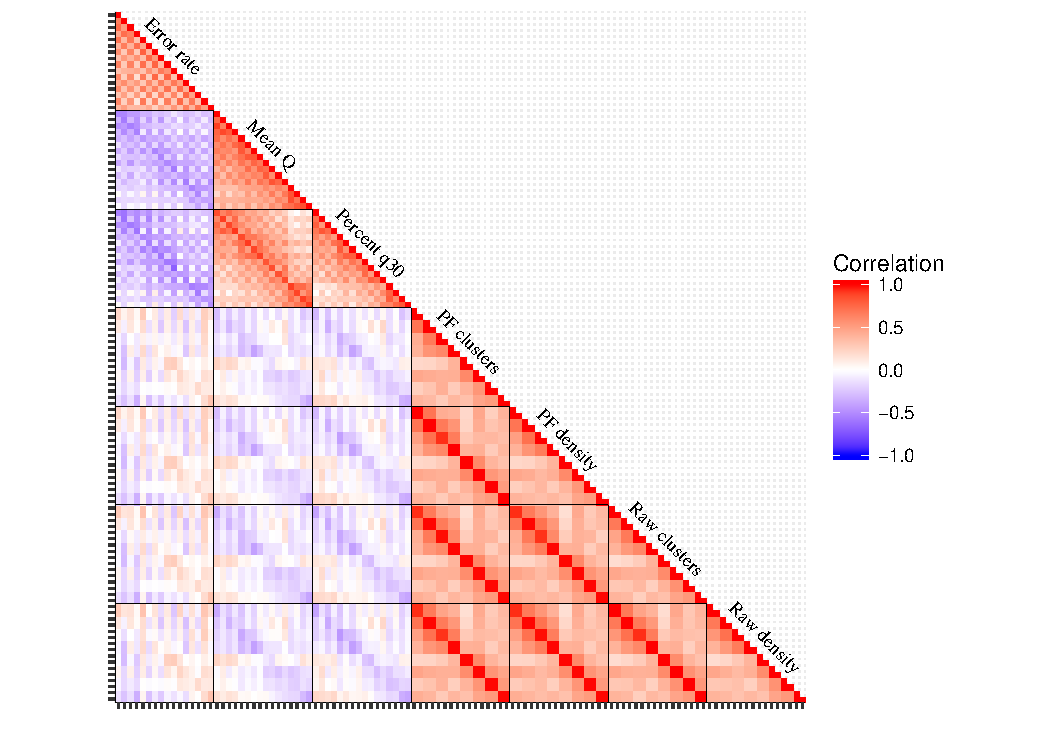
\includegraphics[width=\maxwidth]{figure/ReadlvlCor-1} \caption[Spearman correlation matrix of HiSeq 6 Read level measurements]{Spearman correlation matrix of HiSeq 6 Read level measurements. Two groupings can be seen in the correlation.}\label{fig:ReadlvlCor}
\end{figure}


\end{knitrout}












\chapter{Results}
This section aims to show how the control charts perform in fictive scenarios and practice. The first section will present the calculated control limits and what parameters were used to calculate these. We will introduce the performance measures to be used in this thesis and show how our control charts perform in two simulated scenarios. The last section includes a application on HiSeq quality control data. The control charts will be constructed from the transformed HiSeq 6 quality control data using the transformed mean q, error rate, percent q30 variables. The transformation of the data is described in the Appendix, section \ref{NormalSection}. 
%For the application of the MCUSUM chart we have excluded the HiSeq 3 since it did not have any runs on the same cycle setting. In the application of the MCUSUM charts on the HiSeq 4 and 5 machines we are assuming that the transformed quality control data is generated by the same model we defined in equation \ref{DefCP}. By using the control charts on quality control data in this fashion we are testing if this assumption is true. 




\section{Calculation of control limits}
The number of variables is equal to $p=48$ and the number of observation in the IC sample is equal to $M=73$. Using $\alpha=0.01$, the control limit of Hotelling's $T^2$ is equal to $337.57$. 

To calculate the control limits for the MCUSUM scheme we use the function \texttt{CalculateControlLimit}, described in section \ref{AVERG}. In this thesis we will use a set of allowance constants $k$ to see how the different control charts act with the use of different allowance constants. The following inputs was used in the calculations of the control limits.
\begin{itemize}
\item Allowance constants $k = \{0.30, 0.40, 0.50\}.$
\item Target in-control average run length ARL$^*_0 = 100$.
\item Maximum number of iterations Nmax= 40 or 20.
\item The number $\epsilon$ was set to $0.05$.
\item The number of simulations was set to $10^5$ 
\end{itemize}
The in-control parameters $\boldsymbol{\mu}_0$ and $\boldsymbol{\Sigma}_0}$ were estimated from the transformed data. The constant $a_0$ was set sufficiently small in each simulation to ensure convergence, often close or equal to zero. The upper limit $b_0$ was tailored for each allowance constant, $k$. For $k=0.3$, $b_0$ was chosen large, equal to $1000$ or $10 000$ since no prior information on the control limit is available. In the next calculation with a larger allowance constant $k$, $b_0$ was chosen close to the calculated control limit in previous step with a smaller allowance constant. In Table \ref{Control} the control limits are listed for the mean and covairance chart with the use of different allowance constants. 

% latex table generated in R 3.2.3 by xtable 1.8-2 package
% Mon Jun 13 16:22:24 2016
\begin{table}[ht]
\centering
\caption{The control limits calculated using the function \texttt{CalculateControlLimit} for a set of allowance constants k.\label{Control}} 
\begin{tabular}{lccc}
\toprule
& \multicolumn{3}{c}{$k$} \\ \cmidrule(r){2-4} 
Type & 0.3 & 0.4 & 0.5 \\ 
\midrule
Mean & 2580.242 & 2100.029 & 1713.218 \\ 
\midrule
Covariance & 382.812 & 226.562 & 116.547 \\
\bottomrule
\end{tabular}
\end{table}
\section{Performance measures and simulation study}
We will consider two different out-of-control scenarios. The first scenario will emulate a broken lane, all measurements on this lane will persistently show worse behaviour. The second case considers odd behaviour in the error rate of lane 1, while every other variable is performing as expected. We assume that these scenarios can manifest itself in the mean and the covariance matrix but we will not consider them at the same time. Next we present the performance measures we are going to use. 

\subsection{Perfromance measures}
To evaluate the performance of the charts, two measures will be used. The ARL$_1$, which is described as the time it takes until we discover the change which is present. It is defined in the same manner as the ARL$_0$, i.e.
\begin{align}
&N^*=\inf \{t \in \mathbb{Z}_+: H_t>h \}& \\\nonumber
&\text{E}[N^*] = \text{E}[\inf \{t \in \mathbb{Z}_+: H_t>h \}].& 
\end{align}
Note that we have removed the subscript $h$ and added a star to distinguish between the ARL$_0$ and ARL$_1$. The ARL$_1$ assumes that the machine breaks as soon as we start to monitor the process. For Hotellings $T^2$ we will set a max ARL$_1$ to 500. If Hotellings $T^2$ control chart does not indicate a change after the observations in the out-of-control scenarios we will say that it failed to detect the change.

Now, to assume that the machine breaks as soon as Phase 2 monitoring begins may not be a very realistic case. The conditional expected delay (cf. \cite{ED}) can be used to emulate more realistic cases where changes occur after some time. The conditional expected delay is defined as 
$$
\text{ED}_{\tau}(N^*) = \text{E}_{\tau}[N^*-\tau+1|N^*\geq \tau]
$$
which allows for shifts at arbitrary times $\tau$. In our simulations we will set $\tau=20$. These expectations will be approximated using monte carlo approximation with $10^5$ simulations.

The performance of the change point estimation model will be evaluated using following performance measure
$$
\bar{D}=\frac{1}{n}\sum_{i=1}^n \text{D}_i=\frac{1}{n}\sum_{i=1}^n \left(\hat{\tau}_i-\tau \right)
$$
which will give a indication how how our estimated change point compares to the true value, on average. Since the change point detection model assumed a fixed sample size we will perform the simulations in the following way: 
\begin{itemize}
\item Simulate $\tau=20$ observations according to our in control parameters.
\item Simulate $\lfloor \text{ED}_{\tau}[N^*] \rfloor$ number of observations for the given scenario, size of change and allowance constant. 
\end{itemize}
Here $\lfloor \cdot \rfloor$ is the floor, i.e. we take the closest lowest integer of the conditional expected delay as the number of simulations for a given scenario and size of change. In the simulation of $\bar{D}$ we will use the result of $k=0.3$. 
We will continue with defining these scenarios and how we are going to simulate the performance measures.
\subsection{Simulation study}
Let the observed process $\mathbf{X}_t$ be ordered in the following manner. The first three variables are the mean q, percent q30 and error rate variables from the first lane and read. The second triplet of variables are from the first lane but the second read and so forth. Define the out-of-control mean vector $\boldsymbol{\mu}_1$ and out-of-control covariance matrix $\boldsymbol{\Sigma}_1$ in the following way
\begin{align}
&\boldsymbol{\mu}_1=\boldsymbol{\mu}_0 +\begin{pmatrix} -\delta_1 \\ -\delta_2 \\ \delta_3 \\ -\delta_1 \\ -\delta_2 \\ \delta_3 \\ 0 \\ \vdots \\ 0 \end{pmatrix} & \;\;\;\;\;\;\; & \boldsymbol{\Sigma}_1 = \boldsymbol{\Sigma}_0+\boldsymbol{\Delta} &
\end{align}
where 
$$
\boldsymbol{\Delta}=
\begin{pmatrix} 
\boldsymbol{\Delta}_{1} &\mathbf{0}_{(p-6)\times(p-6)}  \\
\mathbf{0}_{(p-6)\times(p-6)} & \mathbf{0}_{(p-6)\times(p-6)}
\end{pmatrix} &
$$
where $\mathbf{0}_{k\times k}$ is a $k\times k$ matrix with all entries equal to zero. The submatrix $\boldsymbol{\Delta}_{1}$ have dimension $6 \times 6$.   
We will continue with simulating scenario 1 where we assume that quality control data indicates increasingly bad performance in lane 1. 
\subsubsection{Scenario 1 - All quality control variables in lane 1 show increasingly poor behaviour}


In this scenario the quality control data shows persistently worse behaviour. We assume that $\delta_i=\delta>0$ for $i=1,2,3$. We also assume this change manifests in the variance. Therefore, all off-diagonal elemets in $\boldsymbol{\Delta}_1$ are zero and the diagonal elements are equal to a constant $\Delta>0$. These changes will be considered in separate simulation studies. 

In Figure \ref{fig:ARL1MeanCase1} we can see the ARL$_1$ and ED of the MCUSUM for different changes in the mean, for different sizes of $\delta$. Note that the values of $\delta$ are small, this is a result of the scale of the transformed data. The ARL$_1$ goes down quickly for increasing values of $\delta$. The conditional expected delay (ED) is seen to decrease quicker than the ARL$_1$. The value of the allowance constant $k$ does not seem to impact the ARL$_1$ or the ED in scenario 1 for persistent changes in the mean. Hotelling's $T^2$ statistic showed no indication of a change, the smallest out-of-control ARL for all $\delta$ was equal to $500$ for this simulated scenario.
\begin{knitrout}
\definecolor{shadecolor}{rgb}{0.969, 0.969, 0.969}\color{fgcolor}\begin{figure}[!ht]
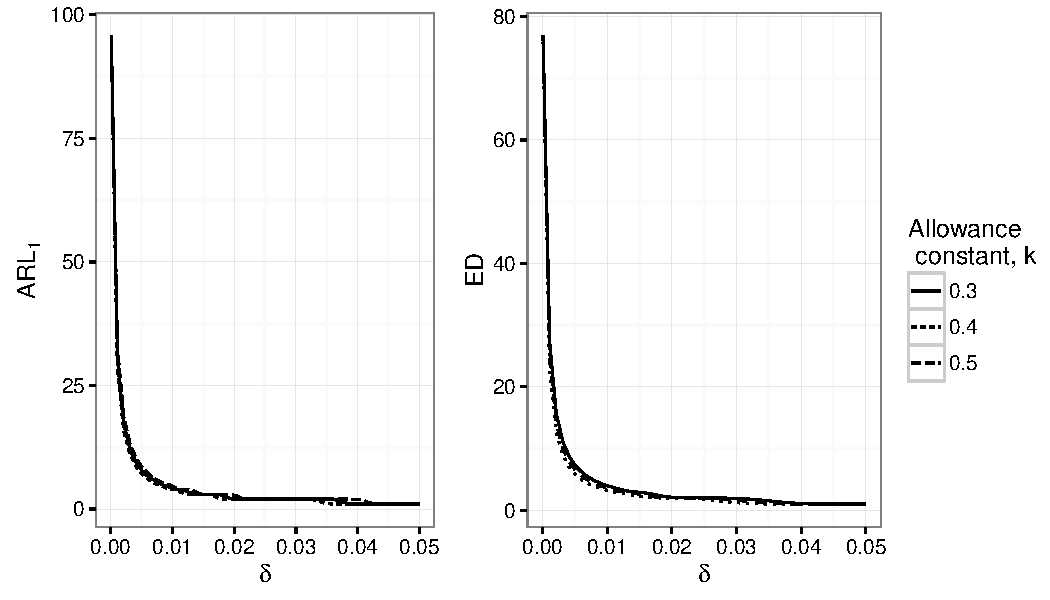
\includegraphics[width=\maxwidth]{figure/ARL1MeanCase1-1} \caption[Out-of-control ARL and ED for the MCUSUM chart of Scenario 1 - changes in the mean of all variables of lane one]{Out-of-control ARL and ED for the MCUSUM chart of Scenario 1 - changes in the mean of all variables of lane one.}\label{fig:ARL1MeanCase1}
\end{figure}


\end{knitrout}


In Table \ref{LongTable1} we have the simulated ARL$_1$ and ED for persistent changes in the covariance matrix. For small changes in the variance of the covariance matrix it takes a long time, on average, to discover the change. As $\Delta$ grows the MCUSUM chart for the covariance matrix detects changes faster. For this specific scenario and shifts the allowance constant $k$ seem to be optimal at $0.5$. The ARL$_1$ and ED is smaller for a allowance constant equal to $0.5$ compared to a allowance constant equal to $0.3$ or $0.4$.
\begin{table}[ht]
\centering
\caption{Scenario 1. MCUSUM simulated out-of-control ARL and ED for changes in covariance matrix. Each cell is on the following form: ARL$_1$ (ED). The ARL$_0$ is equal to 100. $10^5$ replications was used in this simulation study.\label{LongTable1}}
\begin{tabular}{lccccc}
\toprule
& \multicolumn{5}{c}{$\Delta$} \\ \cmidrule(r){2-6}
$k$ & 0.01 & 0.1325 & 0.255 & 0.3775 & 0.5 \\[0.1cm]
\midrule
 0.3 & 92.84 (72.00) & 59.59 (43.69) & 30.55 (23.19) & 18.84 (11.49) & 13.72 (6.84) \\[0.1cm]
\midrule
  0.4 & 94.18 (72.23) &  57.54 (45.90) & 25.71 (21.32) & 14.49 (8.97) & 10.87 (4.44) \\[0.1cm]
\midrule
  0.5 & 87.16 (76.87) & 48.35 (39.75) & 18.11 (12.80) & 10.44 (3.47) & 7.85 (1.10) \\[0.1cm] 
\bottomrule
\end{tabular}
\end{table}

\subsubsection{Scenario 2 - The error rate of lane 1 shows increasingly poor behaviour}

In this scenario we would like to investigate how the charts behave in a situation where only two variables in a lane is effected by some unknown change. In this case we assume that $\delta_1=\delta_2=0$ and $\delta_3>0$. This implies that the error rate increase on average, for lane 1 quality measurements. In the case of changes in the covariance matrix, we assume that the variance will increase and that covariance is held constant. All elements in the matrix $\Delta_1$ are zero except for the third and sixth diagonal element. In Figure \ref{fig:ARL1meanCase2} we can see the ARL$_1$ and ED for the mean in scenario 2. Note that the values of $\delta$ are larger compared to scenario 1. In comparison to scenario 1, it takes a relatively large $\delta$ to discover a change in the error rate variables of lane 1. Hotelling's $T^2$ statistic did not show any indication of a change, the smallest out-of-control ARL for all $\delta$ was equal to $500$.

In table \ref{LongTable2} the results for the ARL$_1$ and ED for simulated changes in the covariance matrix. Here, the value of the allowance constant is seen to have a impact on detecting changes in variance structure of the covariance matrix. The optimal choice of $k$ is equal to $0.5$ for this specific scenario and size of $\Delta$. 

In Table \ref{OffsetTable} we can see the average offset of the change-point estimation procedure for scenario 1 and 2. For increasing values of $\delta$ the estimation procedure becomes more accurate, on average. For small values of $\delta$ we overestimate the change-point. For large values of $\delta$ we start to underestimate the change-point. It should be noted that in cases of large and small $\delta$ we have a very unbalanced sample. 

\begin{knitrout}
\definecolor{shadecolor}{rgb}{0.969, 0.969, 0.969}\color{fgcolor}\begin{figure}[!ht]
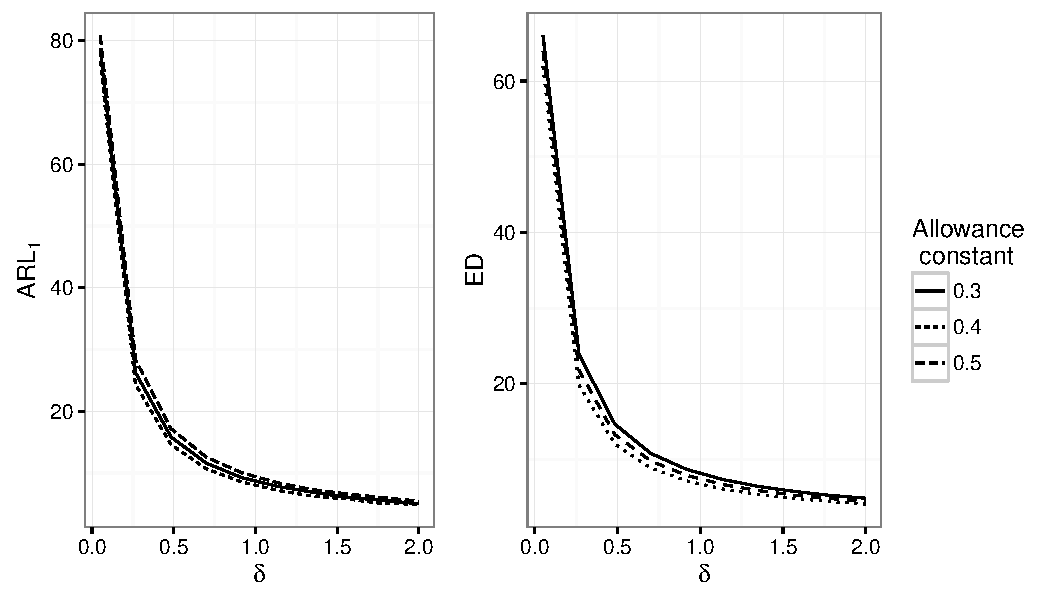
\includegraphics[width=\maxwidth]{figure/ARL1meanCase2-1} \caption[Out-of-control ARL simulations of Scenario 2 - changes in the mean of the error rate of lane one]{Out-of-control ARL simulations of Scenario 2 - changes in the mean of the error rate of lane one.}\label{fig:ARL1meanCase2}
\end{figure}


\end{knitrout}



\begin{table}[ht]
\centering
\caption{Scenario 2. MCUSUM simulated out-of-control ARL and ED for changes in covariance matrix. Each cell is on the following form: ARL$_1$ (ED). The ARL$_0$ is equal to 100. $10^5$ replications was used in this simulation study.\label{LongTable2}}
\begin{tabular}{lccccc}
\toprule
& \multicolumn{5}{c}{$\Delta$} \\ \cmidrule(r){2-6}
$k$ & 0.05 & 0.6625 & 1.275 & 1.8875 & 2.5 \\[0.1cm] 
\midrule
 0.3 & 94.45 (74.05) & 70.15 (51.24) & 49.53 (34.93) & 35.46 (23.63) & 26.87 (16.88) \\[0.2cm]
\midrule
  0.4 & 95.46 (73.17) & 68.24 (49.39) & 46.28 (31.53) & 30.98 (19.90) & 22.21 (12.89) \\[0.2cm] 
\midrule
 0.5 & 88.29 (66.32) & 58.54 (42.01) & 37.56 (23.46) & 22.31 (12.33) & 15.44 (6.60) \\[0.2cm] 
\bottomrule
\end{tabular}
\end{table}

\begin{table}[ht]
\centering
\caption{Table containing $\bar{D}$ for both scenarios. 20 in control observations was used together with a allowance constant of $0.3$.\label{OffsetTable}}
\begin{tabular}{lcccccccccc}
\toprule
\textbf{Sc. 1} & \multicolumn{10}{c}{$\delta$} \\ \cmidrule(r){2-11} 
 & 0.0001 & 0.0052 & 0.0103 & 0.0164 & 0.0215 & 0.0276 & 0.0327 & 0.0388 & 0.0439 & 0.0500 \\ 
 $\lfloor ED \rfloor$ & 76 & 7 & 3 & 2 & 2 & 1 & 1 & 1 & 1 & 1 \\
 $\bar{D}$ & 42.63 & 6.43 & 0.29 & -0.06 & -0.21 & -0.24 & -0.41 & -0.88 & -1.77 & -1.63 \\[0.1cm]
\midrule
\textbf{Sc. 2} & \multicolumn{10}{c}{$\delta$} \\ \cmidrule(r){2-11} 
 & 0.05 & 0.27 & 0.48 & 0.70 & 0.92 & 1.13 & 1.35 & 1.57 & 1.78 & 2.00 \\
 $\lfloor ED \rfloor$ & 65 & 23 & 14 & 10 &  8 &  7  & 6  & 5 & 5 & 4 \\
$\bar{D}$ & 41.65 & 5.60 & 0.20 & -0.04 & -0.13 & -0.17 & -0.31 & -0.75 & -1.64 & -1.53 \\
\bottomrule
\end{tabular}
\end{table}
% \subsection{Robustness (optional section)}
% \begin{enumerate}
% \item What happens under the t-distribution or maybe something skew? 
% \item What happens when the mean and/or covariance matrix is wrongly estiamted? How does this effect control limits etc? 
% \end{enumerate}

\section{A application on HiSeq quality control data.}





In this section we will test the control charts which were constructed from transformed quality control HiSeq 6 on the three other HiSeq machines, namely HiSeq 3, 4 and 5. First, we transform the quality control data from HiSeq 3, 4 and 5 using the Box-Cox transformation with the estimated parameters from the HiSeq 6 data. For variables with limited support, we use the quantile normal function to transform the data. After the transformation we test the constructed control charts on the new data. Any alarm that is given will only be a indication that the in-control parameters for HiSeq 6 does not fit the other machines. 
The HiSeq 3 machine has no runs on the same type of setting which we used for estimating our HiSeq 6 in-control parameters. The data from the HiSeq 3 machine is performed on a mixture of settings. The HiSeq 4 and 5 machines have runs performed on the same setting as those on HiSeq 6.



We will use a allowance constant $k=0.3$ for both MCUSUM charts. The control limits can be seen in Table \ref{Control} for the mean and covariance chart, respectively.

In Figure \ref{fig:HiSeqPhase2Hotelling} we can see Hotellings $T^2$ statistic of the transformed HiSeq 3, 4 and 5 quality control data. Here, a $\alpha=0.01$ was used for calculating Hotelling's $T^2$ statistic control limit, defined in \eqref{HotControlLimit}. Hotelling's control limit was calculated to $337.57$. First, notice the scale of the y-axis. The HiSeq 3 machine was run under different settings which is clearly seen in the left figure of Figure \ref{fig:HiSeqPhase2Hotelling}. Almost all observations are well above the control limit. The first run of HiSeq 3, where Hotellings $T^2$ shows a value of $\ensuremath{2.071688\times 10^{4}}$, stands out in terms of great quality measurements in lane 7 while having very poor quality measurements in read 2, lane 5 and lane 8. The majority of Hotelling's $T^2$ statistics based on transformed HiSeq 4 and 5 quality control data are below the control limit. These runs seem to lie close to our estimated in control parameters in the transformed space.

\begin{knitrout}
\definecolor{shadecolor}{rgb}{0.969, 0.969, 0.969}\color{fgcolor}\begin{figure}[!ht]
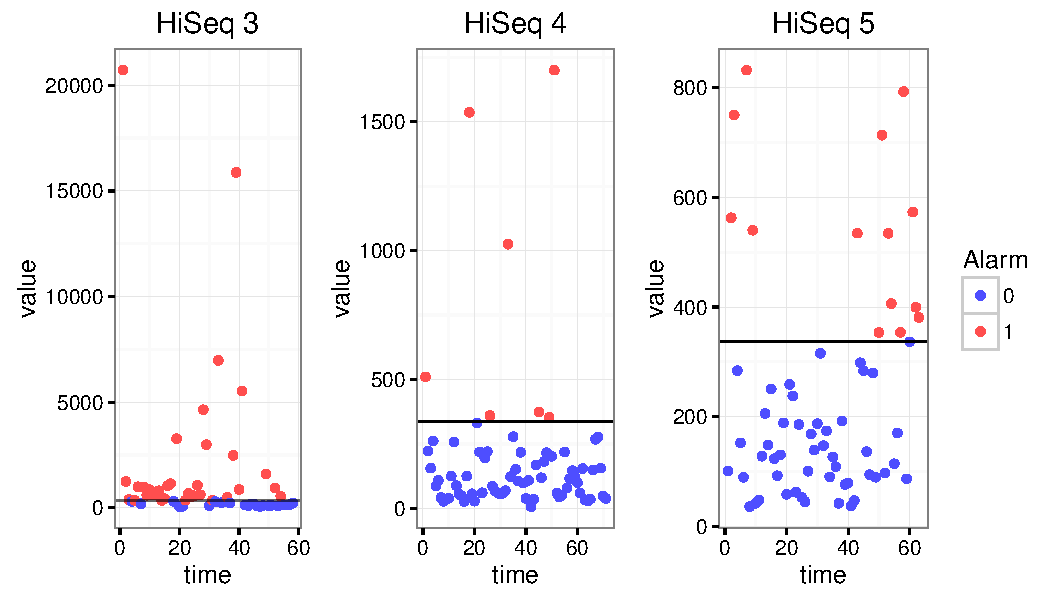
\includegraphics[width=\maxwidth]{figure/HiSeqPhase2Hotelling-1} \caption[Hotellings T-square statistic for the HiSeq 3 (left), HiSeq 4 (middle) and HiSeq 5 machines with in control parameters based on HiSeq 6 data]{Hotellings T-square statistic for the HiSeq 3 (left), HiSeq 4 (middle) and HiSeq 5 machines with in control parameters based on HiSeq 6 data. The straight horizontal line represents the control limit.}\label{fig:HiSeqPhase2Hotelling}
\end{figure}


\end{knitrout}
The MCUSUM charts for the mean vector and covariance matrix are shown in Figure \ref{fig:HiSeq45MCUSUMfig} for the HiSeq 4 and 5 machines. We can see that the charts give a strong indication that the estimated in control mean vector and covariance matrix do not fit the transformed quality data of HiSeq 4 and 5. If we assume that the transformed quality control data for HiSeq 4 and 5 can represent a IC sample from their respective processes, we can calculate the non-centrality parameter, described in section \ref{croiserCUSUM}. Note that we are not removing any observations from the HiSeq 4 and 5 quality control data and that we are using the transformation parameter estimated from HiSeq 6 quality control data. Let $\hat{\boldsymbol{\mu}}_{i}$ be the maximum likelihood estimator of the mean vector based on the $i$-th HiSeq (transformed) quality control data. The non-centrality parameter for HiSeq 4 can be calculated to 
$$
(\hat{\boldsymbol{\mu}}_{0}-\hat{\boldsymbol{\mu}}_{4})\widehat{\Sigma}_0(\hat{\boldsymbol{\mu}}_{0}-\hat{\boldsymbol{\mu}}_{4})'=0.557.
$$
The non-centrality parameter based on HiSeq 5 is calculated to $0.557$. The covariance matrices can be compared using the determinant of the covariance matrices. It represents the squared volume of the parallelotope in $\mathcal{R}^p$ where the eigenvectors are the principal edges (cf. \citet[page 385]{MultStatAnalysis}). The ratio of the determinants serve as a measure of how the squared volume of the parallelotope relates to eachother. Let $\widehat{\Sigma}_i$ be the maximum likelihood estimator based on transformed quality control data from the $i$-th HiSeq machine. Let
$$
R_{i} = \frac{|\widehat{\Sigma}_0|}{|\widehat{\Sigma}_i|}
$$
be the ratio between the in control covariance matrix and the estimated covariance matrix based on the $i$-th HiSeq transformed quality control data. The ratio $R_{i}$ for HiSeq 4 transformed quality control data is equal to $R_{4}=\ensuremath{1.6582958\times 10^{-10}}$ and for HiSeq 5 we have $R_{5}=\ensuremath{1.6582958\times 10^{-10}}$. In the transformed space, these covariance matrices are not equal in terms of their parallelotope volume. Note that this only gives a illustration to whether or not their volume is equal. It does not take the inherent structure of the covariance matrix into account. Also, as described in section \ref{Wishartderiv}, any control chart constructed from the transformed quantities would be sensitive to shifts in the mean. The very large values of the charting statistics, seen in the right column of Figure \ref{fig:HiSeq45MCUSUMfig} could be a result of differences in the covariance matrix \textit{and} the mean vector. Since the charts gave a indication of a change in this manner, the change-point detection model will not be used in this setting.


\begin{knitrout}
\definecolor{shadecolor}{rgb}{0.969, 0.969, 0.969}\color{fgcolor}\begin{figure}[!ht]
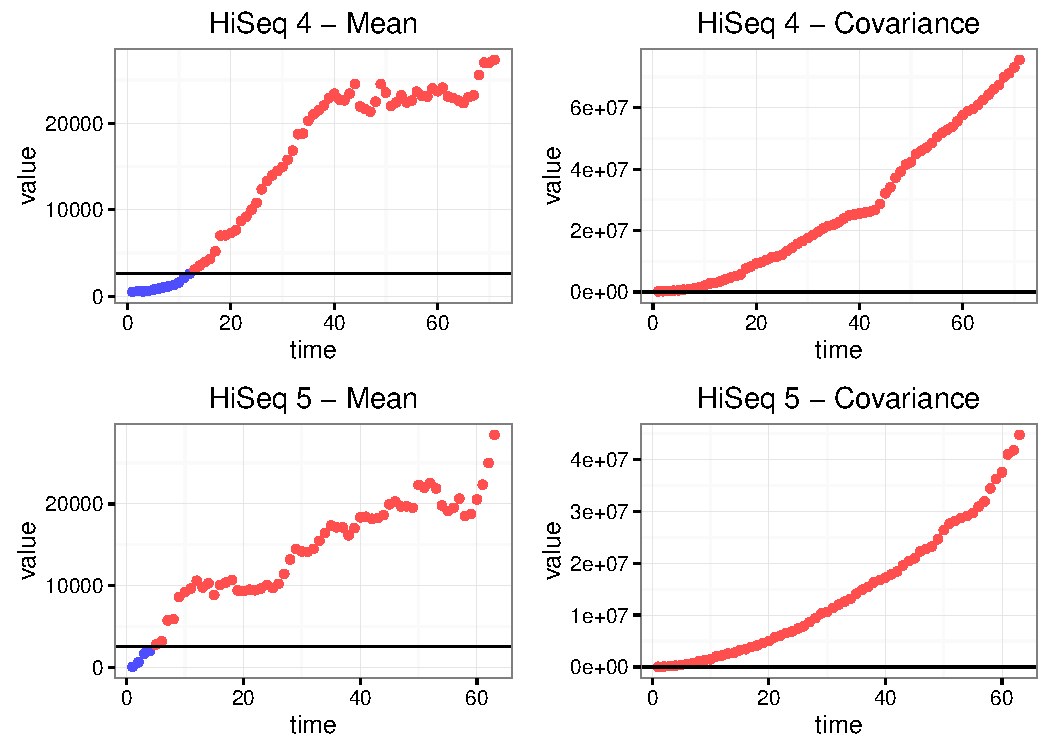
\includegraphics[width=\maxwidth]{figure/HiSeq45MCUSUMfig-1} \caption[MCUSUM control charts monitoring the mean vector and covariance matrix]{MCUSUM control charts monitoring the mean vector and covariance matrix. The in control parameters is based on transformed data from the HiSeq 6 machine. The horizontal line is the control limit calculated with k=0.3.}\label{fig:HiSeq45MCUSUMfig}
\end{figure}


\end{knitrout}


\chapter{Discussion}

In thesis we have investigated how the SPC- and change point detection framework can be used to detect and estimate changes in next generation sequencing quality control data. The control charts presented in this thesis were applied on transformed HiSeq quality control data. The performance of these was tested in a simulation study. Two different scenarios were considered. In scenario one we investigated how quick these charts would detect a change in all variables in a lane. In scenario two we tested how quick the control chart would detect a change in one variable in a lane. Hotelling's statistic was shown to be very poor at detecting small and persistent shifts while the two MCUSUM charts was shown to detect small and persistent changes well. In these two scenarios the change point detection model was shown to be efficient in detecting when the change occurred, if the change was large and the number of runs in OC was relatively short. The number of out-of-control observations used in the estimation was determined by the conditional expected delay. 

We also applied the constructed control charts on other similar machines transformed quality control data. In this application, Hotelling's $T^2$ statistic successfully show differences between runs performed on different cycle settings. It also provides a way to specify the quality limits or control limits from a theoretical point of view. What the Hotelling's $T^2$ statistic failed to detect was the structural changes in quality control data between HiSeq machines. However, one should note that we are using the transformation parameters estimated from HiSeq 6 quality control data to transform the other machines quality control data. 

%The example is not a Phase 2 monitoring example since there may be a numerous of reasons why the charts give a indication of a change. There may be a structural difference between the machines IC parameters and therefore, the signals given by the the two CUSUM charts may be a consequence of this structural difference. The  
% A desirable property is that the HiSeq machines perform in the same manner so the investigation provides some understanding to whether or not these machines are different in the mean vector and covariance matrix. 

%We showed that there was autocorrelation in the data. In \citet{AutoCUSUM} the implications of autocorrelation was investigated in the univariate setting. In this article, they showed that a relatively small autocorrelation can heavily impact the run length distribution. A positive autocorrelation would lead to a decrease in the ARL$_0$. Now, in this specific application the autocorrelation may be somewhat misleading. This assumes that the timeseries which we are investigating is observed at regular intervals. This is not the case. Not only are the machines run at irregular times but the different settings implies that the machine may be used in-between our observations. As an example, according to our model the machine is idle between the $\mathbf{X}_t$ and $\mathbf{X}_{t+1}$ observation. This might be the case, but it can also be that the machine is run on a different setting, which provided different characteristics. A solution is to monitor the grand mean of the error rate or mean q, as an example. In this case we would aggregate all values from different lanes and reads, receiving one observation per variable in each flowcell. We could then adjust for what type of setting the run was performed on. However, this would disregard a possible lane and read effect which may be a large loss of information. 

%In the Literature, there exists non-parametric methods which could be used instead of the charts suggested in this thesis. Assumptions such as the target process should be generated by some symmetric distribution are often made (cf. section 8.2.3 \citet{SPCIntro} or \citet{QuiBoot}). Also, the determination of appropriate control limits is not trivial in this setting. \citet{QuiBoot} suggested a bootstrap procedure to determine the control limits. 

%The change-point estimation model was shown to be ...... However, as described in section \ref{CPDsection}, we refrained from ever estimating a change point of the covariance matrix since the change could only be estimated far back in time. In the event of a change which is discovered  The theory only allows us to consider 
%theory which has been found to determine the control limits in these settings are shown to work through simulations.  
%A example of these are  suggested bootstrap based control limits

In some areas of statistical process control, the mean and covariance structure can be assumed to be known. This is especially true for production processes where one can decide the \textit{desired} mean, variance and covariance structure. In the multivariate setting a new issue arises. Specifying a desired variance for a univariate distribution does not pose a issue but specifying the $p(p+1)/2$ elements in a covariance matrix may be very hard, especially if $p$ is large. Also, the transformation used in this thesis provides several complications. Consider the case when the mean vector is known and is specified in the initial parameter space. We assumed that the transformed data is normally distributed and therefore, we would need to transform the known mean to the new parameter space. The transformation was done by using a Box-Cox transformation, where the parameter $\lambda$ was estimated from data. Any estimate contains uncertainty and therefore the transformation is not deterministic. The problem becomes even more complicated if the parameter $\lambda$ would be random. 

In the Appendix, section \ref{NormalSection} the assumption of normality and temporal independence was investigated. The transformed quality control data showed little evidence of being normally distributed. The evidence shown by these statistical tests could perhaps be increased by further investigating transformation methods. Since there was little evidence for the assumption of normally distributed data any conclusions on temporal independence should be done with great care. However, temporal independence is not only a desirable property for the quality control data but should also be considered a necessary assumption. Not only did the data consist of irregular time series, it was made even more irregular from the different run settings a machine could be run on. Each run setting provided different quality characteristics and dimensionality to the flowcells read level. The autocorrelation assumes that the data are regularly spaced time series, which is not the case. Therefore, using the autocorrelation as a measure of temporal dependency is not only misleading but also violates the assumptions it is built upon.
A solution to this problem is to monitor results quality variables at a flowcell level, aggregating each quality measurements for each read and lane to receive one observation per variable. In this setting one could possibly consider the run settings as fixed, regress upon these fixed settings and then monitor the residuals. 

The use of Rcpp (c.f. \citet{Rcpp}) significantly reduced the time it took to perform the simulations in this thesis. The benchmarks, seen in the Appendix section \ref{Benchmarks}, provide a great indication of how fast Rcpp together with OpenMP can be and what they can do for computer intensive methods in the statistical environment \textsf{R}. \textsf{R} provide a trade-off between performance and readability. The programming language C++ do not follow this paradigm. Rcpp tries to combine these two by using the performance of C++ and the syntax of \textsf{R}. However, it should not be denied that Rcpp is significantly harder to read compared to \textsf{R}.

The 
%For future research another approach to the problem could be useful and perhaps even provide better results. The assumption that each lane and read constitute a random variable correlated with the other variables could be a misinterpretation of the problem itself. What could be more appropriate would be to assume that there exists latent variables. The motivation of latent variables could be as follows, consider a flowcell to be sequenced. The flowcell contains a sample which is \textit{one} source of variation. Second, the machine performs all the sequencing procedures which could be seen as the \textit{second} source of variation. Other sources of variation could also be included, such as a ''human component'' which could be described as the variation coming from the human interaction with the samples. One could then run charts such as those described in this thesis on the .....

%{\Large ToDo}
%\begin{itemize}
%\item what where the assumptions, are they violated? 
%\item shortcomings of the methods? Comment on non-parametric methods.
%\item further research? 
%\item CPD detection shortcomings: \cite{CPDall} the generalized inverse together with a generalized determinant was used to overcome these %shortcomings.
%\end{itemize}

\chapter{Appendix}
\section{Hotelling's $T^2$ statistic}\label{HotDerivation}
In this section we derive the Hotelling's test statistic from the likelihood ratio criterion, as described in \cite{MultStatAnalysis} section 5.2.1. Consider a random sample $\mathbf{X}=\{\mathbf{X}_1, \mathbf{X}_2,...,\mathbf{X}_n\}$ of size $n$, $n>p$, from a p-dimensional normal distribution with mean $\boldsymbol{\mu}$ and covariance matrix $\boldsymbol{\Sigma}$. We want to test the following simple hypothesis
$$
H_0: \boldsymbol{\mu}=\boldsymbol{\mu}_0 \text{  against  } H_1: \boldsymbol{\mu}\neq\boldsymbol{\mu}_0
$$
The likelihood is equal to
$$
L(\boldsymbol{\mu}, \boldsymbol{\Sigma}; \mathbf{X}) = (2\pi)^{-\frac{np}{2}} |\boldsymbol{\Sigma}|^{-\frac{n}{2}} \exp\left(-\frac{1}{2}\sum_{i=1}^n (\mathbf{X}_i-\boldsymbol{\mu})'\boldsymbol{\Sigma}(\mathbf{X}_i-\boldsymbol{\mu})\right)
$$
and therefore the likelihood ratio is equal to
\begin{equation}\label{HotDerivLikRatio}
\lambda = \frac{\max_{\boldsymbol{\Sigma}} L(\boldsymbol{\mu}_0,\boldsymbol{\Sigma)}}{\max_{\boldsymbol{\mu},\boldsymbol{\Sigma}} L(\boldsymbol{\mu},\boldsymbol{\Sigma)}}.
\end{equation} 
Under the null hypothesis the mean vector is known and therefore, the maximum likelihood estimate (MLE) of the covariance matrix is equal to 
$$
\widehat{\boldsymbol{\Sigma}}_0=\frac{1}{n} \sum_{i=1}^{n}(\mathbf{X}_i-\boldsymbol{\mu})(\mathbf{X}_i-\boldsymbol{\mu})'
$$
and under the alternative hypothesis, MLE for mean vector and covariance matrix are given by
\begin{align}
\hat{\boldsymbol{\mu}}&=\bar{\mathbf{X}}=\frac{1}{n} \sum_{i=1}^{n} \mathbf{X}_i&\nonumber \\
\widehat{\boldsymbol{\Sigma}}_1&=\frac{1}{n}\sum_{i=1}^{n}(\mathbf{X}_i-\hat{\boldsymbol{\mu}})(\mathbf{X}_i-\hat{\boldsymbol{\mu}})'= & \label{step1} \\
&=\frac{1}{n}\left(\sum_{i=1}^{n}(\mathbf{X}_i-\boldsymbol{\mu}_0)(\mathbf{X}_i-\boldsymbol{\mu}_0)+n(\bar{\mathbf{X}}-\boldsymbol{\mu}_0)(\bar{\mathbf{X}}-\boldsymbol{\mu}_0)'\right) & \label{step2}
\end{align}
where we have used lemma 3.2.1 from \cite{MultStatAnalysis} to go from equation \eqref{step1} to \eqref{step2}. 
By Lemma 3.2.2, \cite{MultStatAnalysis} page 69, we have that the numerator and denominator in \eqref{HotDerivLikRatio} is equal to
\begin{align*} 
&\max_{\boldsymbol{\Sigma}} L(\boldsymbol{\mu}_0,\boldsymbol{\Sigma)}=(2\pi)^{-\frac{np}{2}} |\widehat{\boldsymbol{\Sigma}}_0|^{-\frac{n}{2}} \exp\left(-\frac{1}{2}pn\right)& \\ 
&\max_{\boldsymbol{\mu},\boldsymbol{\Sigma}} L(\boldsymbol{\mu},\boldsymbol{\Sigma)}=(2\pi)^{-\frac{np}{2}} |\widehat{\boldsymbol{\Sigma}}_1|^{-\frac{n}{2}} \exp\left(-\frac{1}{2}pn\right). & 
\end{align*}
The maximized likelihoods are proportional to each other and therefore the likelihood ratio in equation \eqref{HotDerivLikRatio} reduces to 
\begin{align}
\lambda&=\frac{|\widehat{\boldsymbol{\Sigma}}_0|^{-\frac{n}{2}}}{|\widehat{\boldsymbol{\Sigma}}_1|^{-\frac{n}{2}}}& \nonumber \\
&=\frac{|\mathbf{V}|^{-\frac{n}{2}}}{|\mathbf{V}+n(\bar{\mathbf{X}}-\boldsymbol{\mu}_0)(\bar{\mathbf{X}}-\boldsymbol{\mu}_0)'|^{-\frac{n}{2}}}& \label{HotDerivLikRatioREDUCED}
\end{align}
where $\mathbf{V}=\sum_{i=1}^{n}(\mathbf{X}_i-\boldsymbol{\mu}_0)(\mathbf{X}_i-\boldsymbol{\mu}_0)'$. Before continuing with the derivations we introduce the following Corollary presented in \citet{MultStatAnalysis} page 638

\textbf{Corollary 1.} \textit{For a non-singular matrix }$\mathbf{C}$ \textit{the following holds}
$$
\begin{vmatrix}
\mathbf{C} & \mathbf{y} \\
\mathbf{y}' & 1
\end{vmatrix} = |\mathbf{C}-\mathbf{y}\mathbf{y}'|=
\begin{vmatrix}
1 & \mathbf{y}' \\
\mathbf{y} & \mathbf{C} 
\end{vmatrix} = |\mathbf{C}|(1-\mathbf{y}'\mathbf{C}^{-1}\mathbf{y})
$$
\textit{where }$\mathbf{y}$\textit{ is a p-dimensional column vector.}

Now, let $\mathbf{C}=-\mathbf{V}$ and $\mathbf{y}=\sqrt{n}(\bar{\mathbf{X}}-\boldsymbol{\mu}_0)$, then by Corollary 1 we have that 
$$
|\mathbf{V}+n(\bar{\mathbf{X}}-\boldsymbol{\mu}_0)(\bar{\mathbf{X}}-\boldsymbol{\mu}_0)'| = \begin{vmatrix}
-\mathbf{V} & \sqrt{n}(\bar{\mathbf{X}}-\boldsymbol{\mu}_0) \\
\sqrt{n}(\bar{\mathbf{X}}-\boldsymbol{\mu}_0)' & 1
\end{vmatrix} = |\mathbf{V}|(1+n(\bar{\mathbf{X}}-\boldsymbol{\mu}_0)'\mathbf{V}^{-1}(\bar{\mathbf{X}}-\boldsymbol{\mu}_0)).
$$
Rewrite equation \eqref{HotDerivLikRatioREDUCED} to
\begin{align}
\lambda^{2/n} &= \frac{|\mathbf{V}|}{|\mathbf{V}+n(\bar{\mathbf{X}}-\boldsymbol{\mu}_0)(\bar{\mathbf{X}}-\boldsymbol{\mu}_0)'|} \nonumber \\ 
&= \frac{|\mathbf{V}|}{|\mathbf{V}|(1+n(\bar{\mathbf{X}}-\boldsymbol{\mu}_0)'\mathbf{V}^{-1}(\bar{\mathbf{X}}-\boldsymbol{\mu}_0))}  \nonumber \\
&= \frac{1}{1+n(\bar{\mathbf{X}}-\boldsymbol{\mu}_0)'\mathbf{V}^{-1}(\bar{\mathbf{X}}-\boldsymbol{\mu}_0)}  \nonumber \\
&= \frac{1}{1+T^2/(n-1)} \label{HotDerivLik} 
\end{align}
where 
\begin{align*}
T^2&=(n-1)n(\bar{\mathbf{X}}-\boldsymbol{\mu}_0)'\mathbf{V}^{-1}(\bar{\mathbf{X}}-\boldsymbol{\mu}_0).& 
\end{align*}
The likelihood ratio, equation \eqref{HotDerivLik}, is then compared to a critical region $\lambda\leq\lambda_0$ is chosen such that it results in the desired significance level, under the assumption that the null is true. Since $\lambda_0$ is a real number for us to chose such that the critical region has the right significance level we chose the following 
$$
\lambda_0= \frac{1}{1+T_0^2/(n-1)}\;\; \iff \;\; T_0^2 = \frac{n-1}{ \lambda_0^{-2/n}-1}.
$$
We can now compare Hotelling's $T^2$ statistic to its quantile $T^2_0$. This shows that Hotellings $T^2$ statistic can be derived from a likelihood ratio test. 
\newpage
\section{Transformation, normal assumption and autocorrelation.}\label{NormalSection}




In this section we will present the transformation methods and evaluate the assumption that the process follows a multivariate normal distribution. We will also look upon the autocorrelation and to what extent it is present in the data. However, the autocorrelation should be interpreted with caution. Not only does the assumption of temporal independence depend upon the normality assumption but it also assumes that the timeseries is regular. 

For the variables which have support on the positive real line we will use the Box-Cox transformation, presented in \citet{BoxCox}, i.e.
$$
Z=
\begin{cases}
\frac{X^{\lambda}-1}{\lambda} & \text{for } \lambda \neq 0 \\
\log(X) & \text{else}.
\end{cases}
$$
for transformation. The variables are transformed independently. The parameter $\lambda$ is estimated using the method suggested in \citet{Gurrero}. The Box Cox transformation and the guerro estimation method is implemented in the \texttt{forecast} package. For variables which have limited support on $(0,1)$ we will use the standard normal quantile function as a transformation method. Consider X having support on (0,1), then we have that
$$
Z = \Phi^{-1}(X),
$$
where Y will follow a normal distribution.

Two statistical tests of the normal assumption are presented in Table \ref{TestTable}, performed on the transformed data. Henze-Zirkler's multivariate test of normality, presented in \citet{HenzeZirkler}, shows some evidence against the null that data is not normally distributed. The genaralized Shapiro-Wilk test of normality, presented in \citet{GenShapWilk}, shows no evidence at all.
% latex table generated in R 3.2.3 by xtable 1.8-2 package
% Fri Jun 17 15:22:38 2016
\begin{table}[ht]
\centering
\begin{tabular}{rlr}
  \hline
 & Test & P.value \\ 
  \hline
1 & Henze-Zirkler's & 0.29 \\ 
  2 & Generalized Shapiro-Wilk & 0.00 \\ 
   \hline
\end{tabular}
\caption{Two statistical tests of normality, Henze-Zirkler's and a generalized Shapiro-Wilk's test. One out of two tests approves of the normality assumption.} 
\label{TestTable}
\end{table}

Under the assumption that the transformed data \textit{is} normally distributed, the autocorrelation may be investigated. If the autocorrelation at a given lag is below the standard normal distributions $95\%$ percentile we can assume that the data is independent in time. There are a total of 1128 correlation coefficients at each lag to investigate. We will show the proportion of lags which are greater than the standard normal distributions $95\%$ percentile and all autocorrelation coefficients, for a given lag, in a histogram. 
For the HiSeq 6 machine, the proportion of autocorrelation coefficients greater than the normal quantile are seen in Table \ref{ACFtable} for lags one through five. The autocorrelation for the first two lags are shown in Figure \ref{fig:FigureACF}. Under the assumption of normally distributed data, it can be seen that the HiSeq 6 data shows to much autocorrelation to be independent in a temporal manner. However, since the transformed data shows little evidence that it is normally disitributed, any conclusions on the independence between observations in a temporal manner, could be highly inapproriate and inaccurate. Also, we have removed data before transformation which may have created or removed autocorrelation. 

We will also test the assumption that the estimated covariance matrix is a positive definite matrix using the \texttt{is.positive.definite} function from the \texttt{matrixcalc} package. 

The result from the function is $TRUE$, the estimated covariance matrix is positive definite. 

% latex table generated in R 3.2.3 by xtable 1.8-2 package
% Fri Jun 17 15:22:38 2016
\begin{table}[ht]
\centering
\begin{tabular}{rr}
  \hline
Lag & Proportion \\ 
  \hline
  1 & 0.21 \\ 
    2 & 0.11 \\ 
    3 & 0.05 \\ 
    4 & 0.04 \\ 
    5 & 0.03 \\ 
   \hline
\end{tabular}
\caption{Proportion of autocorrelation greater than the normal 95 percentile, at lags 1 through 5.} 
\label{ACFtable}
\end{table}

\begin{center}
\begin{knitrout}
\definecolor{shadecolor}{rgb}{0.969, 0.969, 0.969}\color{fgcolor}\begin{figure}[!ht]
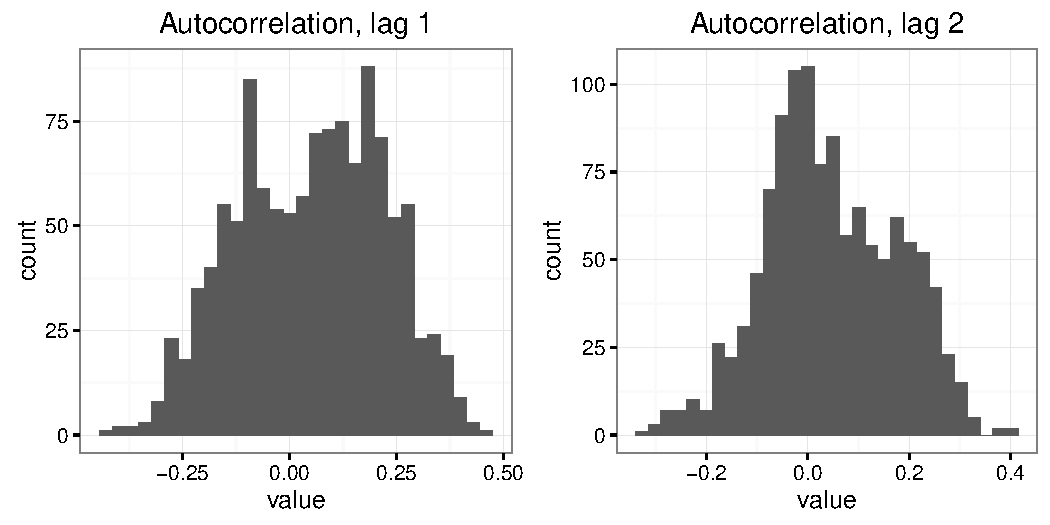
\includegraphics[width=\maxwidth]{figure/FigureACF-1} \caption[Distribution of autocorrelation coefficients at lag 1 (left) and lag 2 (right) of the transformed data]{Distribution of autocorrelation coefficients at lag 1 (left) and lag 2 (right) of the transformed data.}\label{fig:FigureACF}
\end{figure}


\end{knitrout}
\end{center}
\newpage
\section{Rcpp, OpenMP and Benchmarks}\label{Benchmarks}



In this section we will shortly show some benchmarks of the \textt{SimulateARL0} function implemented in Rcpp, which is used in to simulate the in control ARL for a given control limit and allowance constant. Almost every function used in simulations are implemented in Rcpp. To create benchmarks we will use the following settings 
\begin{itemize}
\item The in control mean vector and covariance matrix
\item A allowance constant equal to $0.3$
\item The control limit $2580.24$
\item The number of threads was held constant, equal to 7. 
\end{itemize}
The number of simulations N=$\{10^2,10^3,10^4,10^5\}$. Each simulation is performed 10 times and the average time is taken as the benchmark for this specific setting. The test system was a Intel\textregistered Core i7-4770S@3.1Ghz with 16Gb system RAM running Ubuntu 14.04.4. In Figure \ref{fig:BenchmarkFigure} we can see how the average time it takes to perform N simulations. The results are shown on a log 10 scale. It takes around $25.56$ minutes to perform a $10^4$ simulations.
\begin{knitrout}
\definecolor{shadecolor}{rgb}{0.969, 0.969, 0.969}\color{fgcolor}\begin{figure}[!ht]
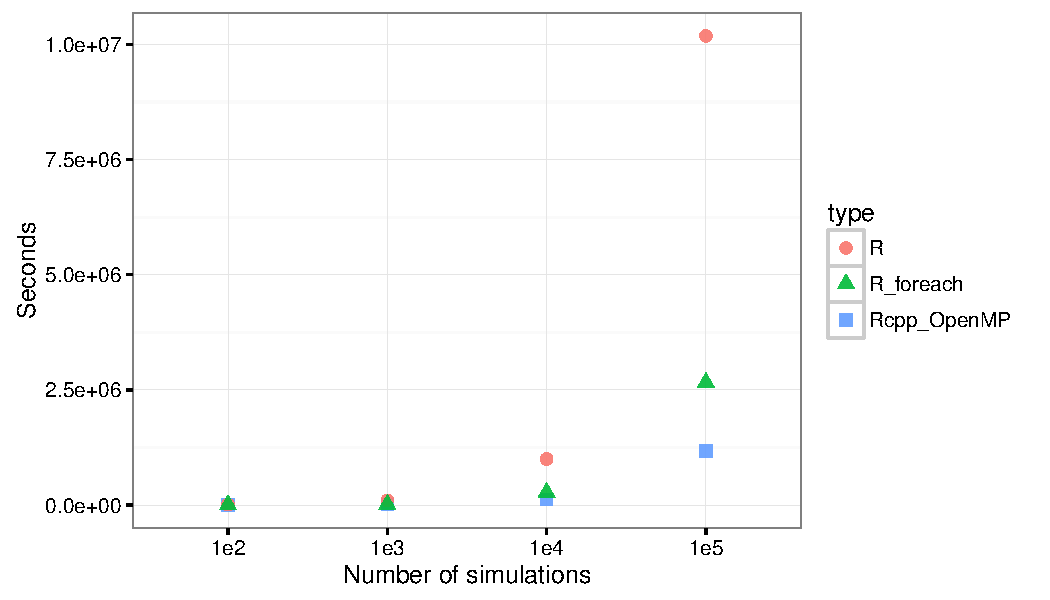
\includegraphics[width=\maxwidth]{figure/BenchmarkFigure-1} \caption[Benchmark of the SimulateARL0 function, implemented in Rcpp together with OpenMP]{Benchmark of the SimulateARL0 function, implemented in Rcpp together with OpenMP. }\label{fig:BenchmarkFigure}
\end{figure}


\end{knitrout}
{\Large Present Rcpp code here? Will get very messy!}

%The Rcpp code for the \texttt{SimulateARL0} function is presented below. The functions \texttt{SnewFun} and \texttt{CFun} calculates $S_{t+1}$ and $C_t$ respectively.\textit{THIS GETS VERY MESSY. REMOVE?}

\newpage

\printbibliography
 
\end{document}
